%
% You may wish to use some of the following options of the iitthesis
% package:
%
% fullpageDraft      avoid the margins necessary for proper binding and
%   just view or print a draft.
% beforeDefense      makes the personal acknowledgements invisible;
%   use this to print the copies you submit initially to the grad school
%   for sending to the opponent panel, i.e. thesis readers (who shouldn't
%   see those parts). For the final submission, after having successfully
%   defended - drop this option.
% noabbrevs          no notation & abbreviations list will be included
%   in the thesis.
%
% Additionally, you must specify the degree for which you're writing
% your thesis (MSc/PhD/MArch etc.)
%
% \documentclass[PhD,noabbrevs]{misc/iitthesis}
\documentclass[MSc,fullpageDraft,beforeDefense,noabbrevs]{misc/iitthesis}


% Definitions of info fields for the thesis - subject, advisor,
% faculty, acknowledgements, etc. etc. This file must contain Hebrew
% text, so the question of its character set encoding is significant.
% This templated uses the iso-8859-8-i charset (i.e. single-byte logical 
% Hebrew; it's about the same as the windows-1255 codepage, but not the
% same as UTF-8) - and this works with MikTeX 2.9 and using pdfelatex.
% With your TeX distribution you might need to create files in the
% UTF-8 charset.
%\authorEnglish{Mish Talem}
%\authorHebrew{מש תלם}

%\titleEnglish{Improved algorithms \\ for the cultivation of lettuce \\ on the coastal plane}
%\titleHebrew{אלגוריתמים משופרים \\ לגידול חסה במישור החוף}

%\disciplineEnglish{Computer Science}
%\disciplineHebrew{מדעי המחשב}

\supervisionEnglish{This research was carried out under the supervision of Prof.~Big Shot, in the Faculty of Computer Science.}
\supervisionHebrew{המחקר בוצע בהנחייתו של פרופסור אישחשוב עצמוני, בפקולטה למדעי המחשב.}

\GregorianDateEnglish{January 2012}
% In Hebrew-language text with babel, if you use a number, the digit order
% gets reversed; if you \L{123} it, you get the number in the English-language
% font glyphs for numbers. Instead, use \beginL 123 \endL - which only changes
% the direction, not the language
\GregorianDateHebrew{ינואר \beginL 2012 \endL}
\JewishDateEnglish{Tevet 5772}
\JewishDateHebrew{טבת התשע"ב}

%\financialAcknowledgementEnglish{The Technion's funding of this research is hereby acknowledged.}
%\financialAcknowledgementHebrew{הכרת תודה מסורה לטכניון על מימון מחקר זה.}

\publicationInfoEnglish{%
% The following may not be true regarding your own thesis...
(The grad school guidelines now require that you mention the following regarding publications of your thesis work; but of course, remove this parenthesized note...; this is to be found in the \texttt{thesis-fields.tex} file. Note also that the document may need to be processed several times before the list of publications actually appears)
Some results in this thesis have been published as articles by the author and research collaborators in conferences and journals during the course of the author's doctoral research period, the most up-to-date versions of which being:

% No need to specifically non-cite the items, all of the bib file's contents
% will appear here regardless
%\nociteacks{firstwork-foracks}
%\nociteacks{secondwork-foracks}
\butcheredbibliography{pubinfo}{front/pubinfo}
}

\publicationInfoHebrew{%
)התייחסות לפרסומים, שמופיעה להלן, הינה הכרחית לפי תקנות ביה"ס ללימודי מוסמכים; כמובן שיש למחוק את ההערה הזו שבסוגריים... תוכן זה נמצאה בקובץ \L{\texttt{thesis-fields.tex}}. כן ייתכן שיהיה צורך להדר את המסמך פעם או פעמיים נוספות עד שהרשימה אכן תופיע כראוי.(
חלק מן התוצאות בחיבור זה פורסמו כמאמרים מאת המחבר ושותפיו למחקר בכנסים ובכתבי-עת במהלך תקופת מחקר הדוקטורט של המחבר, אשר גרסאותיהם העדכניות ביותר הינן:%

\begin{otherlanguage}{english}%
% No need to mention the bibliography file this time, as it has already been used in
% the English invocation
\butcheredbibliography{pubinfo}{front/pubinfo}
\end{otherlanguage}%
}

\thesisbibfiles{back/general.bib,misc/LocalBib.bib}
\thesisbibstyle{plain}


% Personal acknowledgements (are only used for the post-exam
% version)
\personalAcknowledgementEnglish{
I would like to thank my advisor, my parents, my friends, etc. etc.

Add any thank-yous, acknowledgements, personal comments you wish to make here (in \texttt{personal-acks.tex}).

Note that this acknowledgements section only gets printed in the post-exam version of the thesis (i.e. if you leave out the \texttt{beforeDefense} option to your document class in \texttt{thesis.tex}.)
}

\personalAcknowledgementHebrew{

אני רוצה להודות למנחה שלי, להוריי, לחבריי, וכו' וכו'.

אפשר להוסיף עוד תודות והערות אישיות כאן.

שים/י לב: קטע זה של תודות מודפס בפועל רק בגרסת החיבור שלאחר-הבחינה (הווה אומר רק אם הסרת את האפשרות \textenglish{\texttt{beforeDefense}} מן האפשרויות המועברות ל-\textenglish{\texttt{document class}} בקובץ \textenglish{\texttt{thesis.tex}}.)
}


% The abstract in Hebrew and in English should have its own file.
%
% Notes:
% - You can split this one, and have separate files for the English
%   and the Hebrew abstract
% - regulations require the English abstract contain between 200 and
%   500 words, and the Hebrew abstract contain between 1,000 and 2,000
%   words (making it something between an abstract and an introduction
%   with an overview of results).
% - Be careful with links in Hebrew text (wrap them in \L{}).
% Just write down your abstract here, no special commands necessary except for the \abstractEnglish{
% before this text is used and a closing } at the end of it

\abstractEnglish{
% State-of-the-art array processing methods, ranging from high-order statistics to adaptive configuration, require costly computing efforts in pursuit for spatial performance improvement.
The general field of array processing has been thoroughly studied throughout several decades.
The array sensors' spatial diversity enables the extraction of spatial information about impinging signals, thus laying the ground for wide range of applications.
The array size and the number of its elements ($N$) has significant influence on the obtained array performance, such as SNR improvement, spatial separation capabilities and its spatial response's degrees of freedom (DOF).
\par 
Considering localization related applications, several processing approaches are to be found. The most basic approach is \emph{beamforming}, i.e steering the array to different parts of the arena in search of objects.
Another approach, which is probably the most commonly used, is the subspace-based processing which tries to identify input signals that fit into the array's manifold using the orthogonal projection concept.
Statistical processing, although costly in terms of computation effort, is also in use, ranging from maximum-likelihood (ML) related schemes to higher-order-statistics (HOS) using cumulants.
Newer approaches which are still in research stage use neural networking and sparsity-based algorithms.
\par
Although much researched, in this work we revisit the \emph{beamforming} approach.
ULA based beamforming and temporal finite impulse response (FIR) filtering are mathematically analogous, where the DOA acts as the spatial version of temporal frequency.
Inspired by this analogy, we search for the spatial counterpart of the temporal infinite impulse response (IIR) filter.
To this end, we arbitrarily choose to use localization related problem formulation and suggest a feedback based approach, featuring low complexity and high spatial performance in the mere excess of integrating a transmitter to the array.
Considering RADAR-like arrays, the transmitter is already in place, hence a mere processing modification suffices.
Assuming the target of interest has a mirror-like behaviour (i.e., reflects its impinging signals), the spatial feedback between the array and the target is created by continuously re-transmitting a synthesized version of the impinging signal (and its reflections) to the target.
Hence a spatial loop is created, which is shown to be equivalent of enlarging the array's aperture in terms of spatial resolution.
Also notable is that the achievement of the exclusive IIR-like beampattern is purely done in the spatial domain while avoiding any temporal processing to the signal.
\par 
Using a traditional beamforming performance analysis, the beamwidth, peak to side-lobe ratio, array directivity and white noise sensitivity are evaluated for the feedback based array.
A significant improvement in all aspects is shown, while thoroughly discussing the conditions for enhanced performance.
Considering ideal scenarios, the feedback beamformer virtually achieves an infinite aperture, increasing the available spatial information about the target and significantly improves the array's spatial performance.
\par
Taking into account the unavoidable estimation errors and uncertainties, we find that the basic feedback integrated beamformer is very sensitive to even mild range errors.
% Also, the system is more sensitive as the carrier frequency increments.
% Considering practical carrier frequencies, the range sensitivity is of wavelength order. 
% Seeking for a solution, bearing in mind that summing multiple harmonics produce also other lower / higher frequencies, we propose a practical and robust implementation of the feedback-based localization concept.
As a solution, we propose a more complex architecture, using two harmonics, which we call \emph{dual-frequency feedback beamformer}.
We also thoroughly analyse the proposed solution and find that it features low and controllable estimation errors sensitivity in the mere expense of doubling the computation effort.

% At this point you write the abstract of your work, in the main language in which it is written (in this template - English). Graduate school regulations require the abstract to constitute an independent whole and be understood to a reader with general knowledge of the field. Use complete sentences and make few or no citations. Do not refer to the main body of the work and do not use uncommon shorthand, symbols and terms unless you have room for explaining them. The English abstract should be between 200 and 500 words long.

% So this should contain a few more paragraphs...

% \lipsum[10-12]

}

% Note that various commands don't work that well in Hebrew. Specifically,
% if you're using hyperref, you'll have trouble with \url, \autoref, \cite
% and friends. iitthesis-extra.sty has a workaround: the \disabledlinksL
% command. See the .sty for details, or:
% http://tex.stackexchange.com/q/32466/5640 for

\abstractHebrew{

% כאן יבוא תקציר מורחב בעברית (כאשר שפת החיבור העיקרית היא אנגלית). היקף התקציר יהיה \textenglish{1000-2000} מילים. התקציר יהווה שלמות בפני עצמו ויהיה מובן לקורא בעל ידיעות כלליות בנושא.

% בית הספר ללימודי מוסמכים מנחה מספר הנחיות לגבי התקציר בעברית:
% \begin{itemize}
% \item על התקציר להיכתב במשפטים מקושרים שלמים.
% \item בדרך-כלל אין לציין בתקציר מקורות ספרותיים וציטוטים.
% \item אין להתייחס למספר של פרק, סעיף, נוסחה, ציור או טבלה שבגוף החיבור, ואין להשתמש בקיצורים, סמלים ומונחים לא מקובלים, אלא אם יש בתקציר די מקום לזיהויים.
% \end{itemize}

% לעתים יש בכל-זאת יש צורך לכלול פקודה הכוללת קישור פנימי או חיצוני בתוך התקציר העברי; במצבים כאלו כדאי דרך-כלל לעטוף את הפקודה היוצרת את הקישור בתוך פקודת \textenglish{\texttt{\textbackslash{}textenglish\{\}}} כדי למנוע כל מיני פורענויות בלתי-רצויות, כגון כישלון בהידור קובץ ה-\textenglish{PDF} או שימוש בגופן העברי באופן אשר עלול שלא להנעים לעין. לדוגמה: נניח שיש לנו צורך לצטט מקור ביבליוגרפי. אם נעשה זאת סתם-כך: \textenglish{\texttt{\textbackslash{}cite\{Hoeffding\}}}, נקבל: \cite{Hoeffding}; אם נעטוף את פקודת הציטוט, כך: \textenglish{\texttt{\textbackslash{}textenglish\{\textbackslash{}cite\{Hoeffding\}\}}}, נקבל \textenglish{\cite{Hoeffding}} (כפי שהציטוטים נראים גם בטקסט באנגלית).

% \subsection*{\texthebrew{תת-חלק בתקציר המורחב}}

% תוכן מקוצר לגבי נושא מסוים. התייחסות ל\emph{מושג} מסוים שהחיבור בוחן. וכולי וכולי.


% \subsection*{\texthebrew{נקודה מעניינת לגבי העמודים בעברית}}

% שימו לב כי העמודים בעברית אמורים להיות מיוצרים בסדר ה''הפוך'', הווה אומר העמוד האחרון בקובץ ה-\textenglish{PDF} הוא הכריכה העברית, לפניו השער העברי, ודפי התקציר צריכים להופיע בסדר הפוך (וכן במספור רומי, לפי נהלי הטכניון). כך אם נתבונן במספר שבתחתית עמוד זה \textenglish{---} אשר צריך להיות העמוד הראשון בתקציר-המורחב מבחינת רצף התוכן, והינו העמוד האחרון מבין עמודי התקציר-המורחב אחרון בקובץ ה-\textenglish{PDF} \textenglish{---} נמצא את המספר \textenglish{i} ...

% \newpage

% ... ואילו עמוד זה של התקציר-המורחב בעברית \textenglish{---} שהינו העמוד השני בתקציר-המורחב מבחינת רצף התוכן, ונמצא ראשון בקובץ ה-\textenglish{PDF} \textenglish{---} ממוספר ב-\textenglish{ii}. המטרה במספור בסדר ה"הפוך" היא, שבעת ההדפסה לא יהיה צורך להפוך דפים, לשנות את סדרם וכולי \textenglish{---} רק להדפיס ולכרוך.

שיערוך מאפיינים מתוך מדידות הינו מושא לעניין רב עוד מראשית ימי המדע, כשחוקי הפיזיקה נלמדו בעזרת תצפיות ומדידות.
עם התקדמות המדע, רמת הדיוק הנדרשת בשיערוך עלתה ובכדי לעקוף את הגבולות התיאורטיים (פורייה למשל), עלה הרעיון לעיבוד מקבילי של מידע ממספר רגשים.
אחד התחומים בהם עלה משמעותית הצורך בדיוק השיערוך, היה העיבוד המרחבי - קרי שיערוך פרמטרים מרחביים מתוך מדידות. 
עדויות לכך ניתן למצוא עוד בתקופת מלחמת העולם השניה בדמות רדאר ה
\textenglish{Mammut}
שנבנה על ידי הגרמנים לזיהוי מוקדם של מטרות טסות בגבהים עד 8 ק"מ ומרחקים של עד 300 ק"מ.
\par
מאז ועד ימינו, עיבוד מערכי רגשים
\textenglish{(sensors arrays)}
התפתח לכדי תחום מחקר הנותן מענה למגוון רחב של בעיות, ביניהן איכון (מערכות רדאר, סונאר ונגזרותיהן) מטרות על סמך אותות שנפלטים או מוחזרים מהן - הנחשבת לותיקה ביותר בתחום.
עם השנים והתקדמות המדע, נעשה שימוש במערכים לפתרון בעיות נוספות.
\par
במערכות תקשורת, הצורך בסינון מרחבי הוא מן המעלה הראשונה, שכן במציאות מרובת המשדרים והמקלטים, במידה ולא היה שימוש במערכים, הפרעות הדדיות היו מונעות את פענוח האות הנקלט. במקביל, לא רק סינון אלא גם הכוונת אלומת השידור הפכה לאפשרית בזכות השימוש במערכי מופע
\textenglish{(phased array)}
ובכך הושגו גם חסכון באנרגית שידור, מניעת הגעת המידע ליעדים בלתי רצויים, חסינות לרעשים ועוד.
\par
מוקד עניין נוסף, הינו האפליקציות הרפואיות שהתאפשרו בזכות השימוש במערכים. 
בדימות רפואית למשל, כדוגמת 
\textenglish{CT, MRI, EEG}
וכו', רופאים מייצרים באופן בלתי פולשני מודלים של פנים גוף האדם המשמשים לפענוח מצבים רפואיים ותכנון מדויק של הליכים - ובכך מונעים סיכון רב מהמטופלים.
\par
בעשורים האחרונים, עם הגחת הטלפונים הניידים לעולם, עלה הצורך בסינון אותות דיבור מתוך בליל מקורות אקוסטיים, שכן הדובר כבר אינו נמצא בין כותלי ביתו בשקט יחסי.
לשם כך, המכשירים הניידים מצוידים במערכי מיקרופונים אשר מסננים את אות הדובר על פי כיוון הגעתו ומאפייניו הסטטיסטיים.
\par
דוגמא מעניינת נוספת בתחום האסטרונומיה, שם נוכחו המדענים כי תצפיות אופטיות מוגבלות ביכולתן ובכמות המידע שניתן להפיק מהן, היא השימוש במערכי אנטנות, הנפרשים על פני שטחים עצומים בכדי לממש טלסקופים רבי עוצמה ודיוק, העושים שימוש באותות אלקטרומגנטיים באורכי גל שלא בתחום הנראה.
\par
ככלל, בין תחומי מחקר אלו, מתקיימת תרומה הדדית רחבת היקף ורב המסקנות העולות מכל תחום בנפרד משמשות בסיס למחקר ופיתוח בתחומים אחרים ולהפך. 
בנוסף, בבסיס כל מגוון תחומי המחקר, ישנו שימוש בתחום מחקר ותיק ועשיר עוד יותר - הוא השימוש במסננים בכדי להפיק את המידע הרצוי (אות או מאפיין) מהאות הנקלט.  
\par
בבסיס תורת הסינון, שתי אבני בניין מרכזיות - קרי שני סוגי מסננים.
האחד, מסנן בעל תגובה להלם סופית 
\textenglish{FIR}
הינו מישקול וסכימת סט דגימות לכדי מוצא "מסונן".
השני לעומת זאת, משתמש בהיזון חוזר, ובכך מייצר תגובה אינסופית להלם - ועל כך שמו
\textenglish{IIR}
.
לשם תכן מסננים מסופק מפרט התגובה בתדר, בו מפורטים התדרים שאמורים לעבור, אלו שאמורים לחוות דיכוי ומידת הדיכוי הרצויה.
על פי מפרט זה, המתכנן בוחר את סוג המסנן ואת המשקלות שבו.
בעוד המסנן בעל התגובה הסופית להלם מאפשר הימנעות מעיוותים באות (תכונת הפאזה הלינארית - קרי ללא דיספרסיה), המסנן בעל התגובה האינסופית מאפשר חיסכון משמעותי (לעיתים בסדרי גודל) במשאבים לשם עמידה במפרט דומה.
איך לכך, בהתאם לאפליקציה ולמפרט, על המתכנן לבחור במסנן המתאים ביותר תוך הבאה בחשבון של כלל השיקולים - משאבים, עלות וכו'.
\par
עד כה, למיטב ידיעתנו, בכל תחומי המחקר המערבים עיבוד מרובה רגשים אבן הבניין היחידה שבשימוש הינה המסנן בעל התגובה הסופית בתדר, שכן בין אם מעורב שידור במערכת (כמו במכם, תקשורת, דימות רפואית וכו') ובין אם לאו, אין היזון חוזר של האות הנקלט חזרה אל מושא המדידה.
עובדה זו עוררה את תהייתנו ובעטייה חיפשנו את המקביל המרחבי למסנן בעל התגובה האינסופית - בכדי ליהנות מהיתרונות שבו.
במהלך המחקר המקדים, נוכחנו לדעת כי שאלה זו התעוררה גם במוחם של חוקרים אחרים, אך לאחר בחינת פרסומיהם נוכחנו כי פתרונם אינו מממש בצורה מלאה את רעיון ההיזון החוזר אלא מנסה למצוא דרכים עקיפות - בכך חושף עצמו לשגיאות ועיוותים משמעותיים.
\par
למשל, עלתה הצעה לשערך את השהיית האות בין רגשים שכנים, וע"י כך לייצר היזון חוזר בצורה מלאכותית.
גישה זו חשופה לשגיאות מדידה וחוטאת למטרת העיבוד המרחבי הטהור - שכן היא מערבת עיבוד זמני.
הצעה נוספת היתה להתייחס לתת מערכים (מתוך מערך אחד) חופפים כאל הסחות זמניות של מערך אחד קטן יותר ובכך לייצר קירוב סופי לתגובת ההלם האינסופית.
הצעה זו אינה אלא פרשנות שונה לעיבוד מבוסס 
\textenglish{FIR}
שכן בסופו של תהליך העיבוד הינו לינארי ומכיל מספר סופי של דגמים במערכת בכל זמן נתון.
שיטה מעניינת, המהווה בסיס למחקר ענף, מטילה את הדגימה המרחבית והדגימה הזמנית אל מישור התדר, בו גל מישורי מיוצג על ידי קו ישר המוטה לפי זוית ההגעה של הגל הפוגע.
בהמשך לכך, מסננים במרחב התדר הדו מימדי מתוכננים על מנת להגביר אותות שמגיעים מכיוונים רצויים.
גישה זו בשימוש רחב בתחום החקר הסיסמי וסובלת בעיקר מחוסר היכולת לתכנן מסננים מדויקים היות והמסננים מחזוריים בתדר, עובדה הגורמת לעיוותים בקצוות מרחב התדר.
עוד על כן, גם שיטה זו אינה סינון מרחבי טהור ולכן אינה מהווה פתרון לשאלת המחקר אותה ניסינו לפתור.
\par
מוצעת איפוא, מערכת מבוססת מערך לינארי בעל מרווחים אחידים בין הרגשים
\textenglish{ULA}
כאשר בראשיתו, בנוסף על הרגש, ישנו משדר.
על פניו, מערכת דומה למכ"ם, הפולט אות ומשערך את מיקומי מטרות על פי האות החוזר.
החידוש בהצעה נעוץ בכך שהאות המשודר אינו רק אות מלאכותי הנוצר ע"י המערכת אלא משולב בו האות המסונן הנקלט ע"י המערך, בכך נוצר היזון חוזר בין מהמערך והמטרה.
ניתוח המערכת מרמז כי ע"י שליטה במשקלות המסנן המייצר את האות החוזר, ניתן להפיק את היתרונות הרבים הטמונים במסנן בעל התגובה האינסופית.
\par
לאחר מכן, הדמיות ובחינה דקדקנית של המערכת מגלים כי המערכת בעלת רגישות גבוהה למדי - אבן נגף משמעותית בנסיון למציאת הפתרון.
עם זאת, לשמחתנו, נמצא גם פתרון פשוט וזול יחסית לבעיה, המגדיל סך הכל את המאמץ החישובי ולא את המערך עצמו.
הדמיות וניתוח נוספים מאשררים כי הפתרון קביל ומשיג תוצאות שבתרחישים אידיאלים נוטות לכדי שלמות.
בנוסף על האיכון הזוויתי שחווה שיפור משמעותי בביצועיו, כתופעת לוואי, מתכנן המערך יכול גם לקבוע גבולות מרחק לסינון ובכך לייצר מערכת איכון שמזהה לא רק כיוון אלא מיקום מדויק של מטרות.


}
% Just write down your abbervations here - or comment-out the command

\abbreviationsAndNotation{
\begin{tabular}{p{2cm}@{:\quad}l}
QED & quod erat demonstratum \\
$c$ & the speed of light \\
$a\pm b$ & the closed interval $\left[a-b,a+b\right]$ \\
\end{tabular}
}


% Additional machinery relevant to any thesis
% (it's not part of the document class because it's not absolutely
% necessary and not everyone might like it)
\usepackage{misc/iitthesis-extra}

% Definitions useful for anything you write, which you also
% include in any articles, presentations, HW assignments and other
% documents. May contains macros for notation algebra, logic,
% calculus and other fields, as well as general shorthands and
% LaTeX tricks, and package use commands
% General-purpose definitions and inclusions
% you are using in any document 
% (regardless of its class and style files used),
% e.g. package uses:

%\usepackage{xspace}

% and macros/command defintions:

%\newcommand{\complexityclass}[1]{{\bf #1}\xspace}
%\newcommand{\NPTIME}{\complexityclass{NP}}

% For this template, we'll only have one single command,
% necessary for including graphics...
\usepackage{graphicx}% http://ctan.org/pkg/graphicx


% Definitions, settings and tweaks for this thesis specifically
% This file should contain your own definitions specific
% only to this thesis;

% What it contains below is used 
% simply for generating dummy text in the sample 
% content provided with the template (see mainchap1.tex);
% so you can safely delete this when creating your own
% thesis
%general:
%Box and color definitions:
%--------------------------
%General definitions:
%-------------------
\newcommand{\etal}{{\em {et al.}}}
% \newcommand{\B}[1]{\mathbf{#1}}
\newcommand{\df}{\triangleq}
\newcommand{\norm}[1]{\left\Vert#1\right\Vert}
\newcommand{\abs}[1]{\left\vert#1\right\vert}
\newcommand{\RE}{\operatorname{Re}}
\newcommand{\IM}{\operatorname{Im}}
\newcommand{\sgma}[3]{\sum\limits_{{#1}={#2}}^{#3}}
\newcommand{\Brace}[1]{\left\{{#1}\right\}} %Braces
\newcommand{\Brack}[1]{\left({#1}\right)} %Brackets
\newcommand{\sBrack}[1]{\left[{#1}\right]} %square Brackets

%\newcommand{\ip}[2]{{\langle{#1},{#2}\rangle}} %inner-product
\newcommand{\ipLW}[3]{{\langle{#1},{#2}\rangle}_{{#3}}} %weighted inner-product

\newcommand{\Tr}[1]{Tr\Brack{#1}}
\newcommand{\Mtr}[2] %short notation for 2x1 Matrix.
{\begin{bmatrix}
  #1 \\
  #2
\end{bmatrix}}
\newcommand{\cMtr}[2] %short notation for 2x1 Matrix with curves.
{\left(
\begin{array}{c}
    {#1} \\
    {#2} \\
\end{array}
\right)}
\newcommand{\Mtrs}[2] %short notation for 2x1 Matrix star (adjoint)
{\begin{bmatrix}
  #1 &
  #2
\end{bmatrix}}
\newcommand{\Mtrt}[3] %short notation for 3x1 Matrix.
{\begin{bmatrix}
  #1 \\
  #2 \\
  #3
\end{bmatrix}}

\newcommand{\Cases}[4]{
\left\{
\begin{tabular}{lcl}
    $#1$ & $=$ & $#2$\\
    $#3$     & $=$ & $#4$
\end{tabular}
\right. }

\newcommand{\und}{\underline} %How lazy can I get?
\newcommand{\ovr}{\overline}
\newcommand{\conj}[1]{{#1}^\ast} %Conjugation


\newcommand{\er}[1]{{(\ref{#1})}} %equation reference

\newtheorem{Lemma}{Lemma}{}
\newtheorem{Prop}{Proposition}{}
% \newtheorem{theorem}{Theorem}{}


\newenvironment{alg}[5]
{
\begin{figure}[htbp]
\begin{center}
\fbox{
  \begin{ColorBoxedminipage}{13cm}
%    \leftline{\color{Black}\bf {#1}}
    {#4}
   \end{ColorBoxedminipage}
   }
\end{center}
  \bcaptionff{#1}{#2}{}{#3}
  \label{#5}
\end{figure}
}{}

%Just body, caption and label.
\newenvironment{algo}[3]
{
\begin{figure}[htbp]
\begin{center}
\fbox{
  \begin{ColorBoxedminipage}{7.5cm}
%    \leftline{\color{Black}\bf {#1}}
    {#1}
   \end{ColorBoxedminipage}
   }
\end{center}
  \caption{#2}
  \label{#3}
\end{figure}
}{}

\newenvironment{BOX}[1]
{
\begin{center}
\fbox{
  \begin{ColorBoxedminipage}{16cm}
%    \leftline{\color{Black}\bf {#1}}
    {#1}
   \end{ColorBoxedminipage}
   }
\end{center}
}{}

\newcommand\vecnot[1]{\boldsymbol{#1}}
\newcommand\optvecnot[1]{\vecnot{#1}_{opt}}

\usepackage{amsmath}
\DeclareMathOperator*{\argmax}{arg\,max}
\DeclareMathOperator*{\argmin}{arg\,min}
%%%%%%%%%%%%%%%%%%%%%%%%%%%%%%%%%%%%%%%%%%%%%%%%%%%%%%
%%%%%%%%%%%%%%      Document flags     %%%%%%%%%%%%%%%
%%%%%%%%%%%%%%%%%%%%%%%%%%%%%%%%%%%%%%%%%%%%%%%%%%%%%%
\def\DEFIncludeAttenuation{}
\def\DEFInclueApplication{}
%%%%%%%%%%%%  Document Code starts here %%%%%%%%%%%%%%

%%%%%%%%%%%%%%    aliases    %%%%%%%%%%%%%%

% \newcommand{\Brace}[1]{\left\{{#1}\right\}}
\newcommand{\dTheta}{\Delta\theta}
\newcommand{\dPhi}{\Delta\phi}
\newcommand{\dThetaO}{\Delta\theta\rBrace{\omega}}
\newcommand{\dPhiO}{\Delta\phi\rBrace{\omega}}
\newcommand{\dThetaHPBW}{\Delta\theta_{\text{HPBW}}}
\newcommand{\dOmega}{\Delta\omega}
\newcommand{\dR}{\Delta{R}}
\newcommand{\dTau}{CHANGE_TO_DPHI}
% \newcommand{\D}[2]{\mathcal{D}\rBrace{#1,#2}}
% \newcommand{\Dp}[2]{\mathcal{D}^{#2}\rBrace{#1}}
\newcommand{\D}[2]{\text{D}\rBrace{#1,#2}}
\newcommand{\Dp}[2]{\text{D}^{#2}\rBrace{#1}}
% \newcommand{\coefSetName}{\text{CB}}
\newcommand{\coefSetName}{\text{CB}}
\newcommand{\vd}{\vecnot{d}}
\newcommand{\vdO}{\vecnot{d}\rBrace{\omega}}
\newcommand{\vdC}{\vecnot{d}^{\ast}}
\newcommand{\vx}{\vecnot{x}}
\newcommand{\vAlpha}{\vecnot{\alpha}}
\newcommand{\vBeta}{\vecnot{\beta}}
\newcommand{\vdI}[1]{\vecnot{d}_{#1}}
\newcommand{\vdHatI}[1]{\hat{\vecnot{d}}_{#1}}
\newcommand{\vdHatIC}[1]{\hat{\vecnot{d}}^{\ast}_{#1}}
\newcommand{\vdTI}[1]{\vecnot{d}^{T}_{#1}}
\newcommand{\gI}[1]{g_{#1}}
\newcommand{\gIHat}[1]{\hat{g}_{#1}}
\newcommand{\phiI}[1]{\phi_{#1}}
\newcommand{\phiIHat}[1]{\hat{\phi}_{#1}}
\newcommand{\vAlphaTI}[1]{\vecnot{\alpha}^{T}_{#1}}
\newcommand{\vAlphaHI}[1]{\vecnot{\alpha}^{H}_{#1}}
\newcommand{\vBetaTI}[1]{\vecnot{\beta}^{T}_{#1}}
\newcommand{\vBetaHI}[1]{\vecnot{\beta}^{H}_{#1}}
\newcommand{\vAlphaI}[1]{\vecnot{\alpha}_{#1}}
\newcommand{\vAlphaCI}[1]{\vecnot{\alpha}^{*}_{#1}}
\newcommand{\vBetaI}[1]{\vecnot{\beta}_{#1}}
\newcommand{\vBetaCI}[1]{\vecnot{\beta}^{*}_{#1}}
\newcommand{\vAlphaIW}[1]{\vecnot{\alpha}_{#1}}
\newcommand{\vBetaIW}[1]{\vecnot{\beta}_{#1}}
\newcommand{\vAlphaC}{\vecnot{\alpha}^{\ast}}
\newcommand{\vBetaC}{\vecnot{\beta}^{\ast}}
\newcommand{\vBetaFB}{\vecnot{\beta}_{\coefSetName}}
\newcommand{\vBetaCFB}{\vecnot{\beta}^{*}_{\coefSetName}}
\newcommand{\vAlphaFB}{\vecnot{\alpha}_{\coefSetName}}
\newcommand{\vAlphaCFB}{\vecnot{\alpha}^{*}_{\coefSetName}}
\newcommand{\vdT}{\vecnot{d}^{T}}
\newcommand{\vxT}{\vecnot{x}^{T}}
\newcommand{\vAlphaT}{\vecnot{\alpha}^{T}}
\newcommand{\vBetaT}{\vecnot{\beta}^{T}}
\newcommand{\vdH}{\vecnot{d}^{H}}
\newcommand{\vdHat}{\hat{\vecnot{d}}}
\newcommand{\vdHatC}{\hat{\vecnot{d}}^{\ast}}
\newcommand{\vxH}{\vecnot{x}^{H}}
\newcommand{\vAlphaH}{\vecnot{\alpha}^{H}}
\newcommand{\vBetaH}{\vecnot{\beta}^{H}}
\newcommand{\vEta}{\vecnot{\eta}}
\newcommand{\vEtaT}{\vEta^{T}}
\newcommand{\vEtaH}{\vEta^{H}}
%\newcommand{\F}[1]{#1^{\mathcal{F}}}
\newcommand{\F}[1]{\text{\MakeUppercase{#1}}}
\newcommand{\ePhi}[1]{\exp{\rBrace{#1j\phi}}}
\newcommand{\thetaD}{\theta_{\text{d}}}
\newcommand{\Hba}{H_{\vBeta,\vAlpha}}
\newcommand{\HbaFB}{H_{\vecnot{\beta}_{\coefSetName},\vecnot{\alpha}_{\coefSetName}}}
\newcommand{\vp}{\vecnot{p}}
\newcommand{\vpi}[1]{\vp_{#1}}
\newcommand{\vpt}{\vp_{\text{t}}}
\newcommand{\Steer}[1]{\vd_{#1}} 
\newcommand{\aTd}{\vAlphaT\Steer{}} 
\newcommand{\aHd}{\vAlphaH\Steer{}} 
\newcommand{\bTd}{\vBetaT\Steer{}}
\newcommand{\bHd}{\vBetaH\Steer{}}
\newcommand{\Hr}{\mathcal{H}}
\newcommand{\HrTPr}{\mathcal{H}_{\Delta\theta,\Delta\phi,r}}
\newcommand{\myTodo}[2]{\ifdefined\showTodo{\todo[#1]{#2}}\fi}
\newcommand{\myTodoNew}[2]{\ifdefined\showTodoNew{\todo[#1]{#2}}\fi}
\newcommand{\Tx}{\text{T}_{\text{x}}} 
\usepackage{xparse}
\usepackage{latexsym}
\usepackage{amsfonts}
\usepackage{graphicx}
\usepackage{txfonts}
\usepackage{wasysym}
\usepackage{enumitem}
\usepackage{adjustbox}
\usepackage{ragged2e}
\usepackage{tabularx}
\usepackage{changepage}
\usepackage{setspace}
\usepackage{hhline}
\usepackage{multicol}
\usepackage{float}
\usepackage{multirow}
\usepackage{makecell}
\usepackage{fancyhdr}
\usepackage[toc,page]{appendix}
\usepackage[T1]{fontenc}
\usepackage{hyperref}
\usepackage{esvect}
\hypersetup{
    colorlinks=true,
    linkcolor=blue,
    filecolor=magenta,      
    urlcolor=cyan,
}
\usepackage{isomath}
\usepackage{fixmath}
\usepackage{tikz}
\usepackage{textcomp}
\usepackage{epstopdf} %converting to PDF
\usepackage{upgreek}
\usepackage{mathtools}
\usepackage{xfrac}
\usepackage{lipsum}
\usepackage[colorinlistoftodos]{todonotes}
\usepackage[percent]{overpic}
\usepackage{stfloats}
\usepackage{subcaption}
\usepackage{longtable}

\DeclareTextCommandDefault{\nobreakspace}{\leavevmode\nobreak\ }

% \usepackage{listings}
% \usepackage{color} %red, green, blue, yellow, cyan, magenta, black, white
% \definecolor{mygreen}{RGB}{28,172,0} % color values Red, Green, Blue
% \definecolor{mylilas}{RGB}{170,55,241}

% \lstset{language=Matlab,%
%     %basicstyle=\color{red},
%     breaklines=true,%
%     morekeywords={matlab2tikz},
%     keywordstyle=\color{blue},%
%     morekeywords=[2]{1}, keywordstyle=[2]{\color{black}},
%     identifierstyle=\color{black},%
%     stringstyle=\color{mylilas},
%     commentstyle=\color{mygreen},%
%     showstringspaces=false,%without this there will be a symbol in the places where there is a space
%     numbers=left,%
%     numberstyle={\tiny \color{black}},% size of the numbers
%     numbersep=9pt, % this defines how far the numbers are from the text
%     emph=[1]{for,end,break},emphstyle=[1]\color{red}, %some words to emphasise
%     %emph=[2]{word1,word2}, emphstyle=[2]{style},    
% }

\usepackage[framed,numbered,autolinebreaks,useliterate]{misc/mcode}

% If you are using WinEdt, and using a publication list on the the
% acknowledgements page, and are having problems getting your document
% to compile with the 'PDFLaTeXify' button, try uncommenting the
% following two lines;
% Also, you will need to PDFLaTeXify at least twice, as WinEdt misses
% an extra run. See also:
% http://tex.stackexchange.com/q/41727/5640
\usepackage{multibib}
\newcites{pubinfo}{Acknowledgement page references}
\def\iitthesisextramultibibdefs{}

\begin{document}

% Front Matter
% ------------

% The following command will typeset the outer cover page, the
% inner title page, the acknowledgements page, etc. - everything
% up to but not including the introduction
\makefrontmatter

% Main Matter
% ------------
%
% To conform to Technion regulations, the main matter should begin
% with an introduction (including a survey of relevant past work):
%
\chapter{Introduction}
\label{chap:intro}
\section{Background and Motivation}
The general field of array processing has been thoroughly studied throughout several decades.
The array sensors' spatial diversity enables the extraction of spatial information about impinging signals, thus laying the ground for wide range of applications, such as localizing a transmitting source \cite{skolnik2008radar,long2019}, blindly separating mixtures of impinging signals \cite{comon1994independent}, improving SNR \cite{verdu1998multiuser}, and many more. 
\par The ULA has always been a point of interest, due to its simplicity of analysis \cite{van2004optimum,benesty2018}. 
The array size and the number of its elements ($N$) have significant influence on the obtained array performance, such as SNR improvement, spatial separation capabilities and its spatial response's degrees of freedom (DOF).
\par Early algorithms for direction of arrival (DOA) estimation were based on the beamforming concept \cite{krim1996two}, where the array's reception beam is steered (mechanically or electronically) to multiple directions in search of received energy peaks which are interpreted as valid emitters.
One notable improvement to the conventional beamformer \cite{van2004optimum} was Capon's beamformer  (aka minimum variance distortionless response (MVDR)) which attempts to minimize the power contributed by noise and any signals coming from other directions than the DOA of interest, while maintaining a fixed gain
in the desired direction.
\par The most practically used approach in DOA estimators, referred as the subspace based estimation, involves invariant subspace analysis of observed covariance matrices.
Early research includes PCA and errors-in-variables time series analysis \cite{krim1996two}.
However, the tremendous interest in the subspace approach is mainly due to the introduction of the
MUSIC (Multiple SIgnal Classification) algorithm \cite{schmidt1986multiple} which decomposes the estimated covariance matrix to its signal and noise eigenvectors, using orthogonal projection exploiting the fact that the noise subspace is orthogonal to the signal subspace.
It is interesting to note that while earlier works were mostly derived in the context of time series analysis and only later applied to the sensor array problems, MUSIC was originally presented as a DOA estimator.
\par A less practical, but optimal in the sense of root mean square error (RMSE) \cite{krim1996two}, is the maximum likelihood (ML) approach which tries to find the most probable DOA assuming a known PDF.
Though this approach served as a basis for extensive research, leading to more advanced concepts such as the independent component analysis (ICA) \cite{hyvarinen1999survey}, in the context of practical DOA estimation it's computational effort is high.
Adding the fact that sub-optimal methods such as MUSIC were proven to achieve the Cram\'er Rao lower bound (CRLB) under some practical assumptions (e.g. non-coherent signals) \cite{stoica1989music}, these sub optimal estimators are substantially more common in practice. 
\par In pursuit of spatial performance improvement, namely higher spatial separation and selectivity of arriving signals, many approaches were suggested.  
One approach, commonly referenced as ``virtual arrays'' \cite{pal2010nested,chevalier2005virtual,dogan1995applications} deals with the extraction of samples originated in sensors that do not really exist, by using high (higher than 2) order statistics and manipulating multiple statistical cross-terms in order to estimate statistical characteristics of signals impinging in missing sensors.
\par Using a similar approach, the $2q$-MUSIC algorithm \cite{chevalier2006high}, enables the use of $N^{2q}$ ``virtual elements'', by calculating the $q$'th order statistics.
Another approach, involving different array geometries, examined minimum redundancy arrays \cite{moffet1968minimum,pillai1985new,pillai1987statistical,Kupershtein2013}, aiming to reduce the spatial ambiguity. The basic concept was minimization of the inter-element spacing redundancy in order to increase the overall resolution.
Although the $q$-th order statistics based approach promises substantial improvement, both noise sensitivity and impractical computation costs are dominant drawbacks, limiting the usage of such methods in practical applications.   
\par Adaptive processing schemes \cite{frost1972algorithm,manolakis2000statistical}, being a wide and active research area, were also suggested trying to adaptively estimate and suppress the noise component in impinging signals by minimization of the receiver's output energy with some constraints.
In \cite{manolakis2000statistical}, two main approaches to adaptive processing are discussed. The block adaptive scheme (which is also called \textit{sample matrix inversion}) and the sample-by-sample method.
In both methods, after a certain amount of time, the system refreshes the spatial filter coefficients, trying to better suppress the received noise.
As in many adaptive processing applications, the two methods rely on steepest descend optimization, which exposes the adaptive processing approach to errors related to optimization parameters choices such step size etc.
\par In \cite{van1988beamforming}, ULA based beamforming and temporal FIR filtering are shown to be mathematically analogous, where the DOA acts as the spatial version of temporal frequency.
Inspired by this analogy, which is thoroughly discussed in Sec.~\ref{sec:prlm_FIR_IIR}, we were motivated to find the spatial counterpart of the temporal IIR filter, both from academic curiousness and due to the known advantages of the IIR filter's performance.
Therefore we formulated a question, ``what are the equivalent spatial domain processing methods which will be analogous to temporal IIR filtering?'' which served as a guide throughout our research.
\par Achieving spatial IIR response has also motivated other works.
In \cite{wen2013extending} two methods were considered.
The first one (see Fig.~\ref{fig_intro_wen1}) was to estimate the time of arrival (TOA) difference between two consecutive sensors and to synthetically generate the recursive part of the IIR filter, entirely in the time-domain.
\begin{figure}[ht!]
    \begin{center}
        \begin{overpic}[width=0.5\linewidth, 
        %grid, 
        tics=10,trim=0 0 0 0]{./Media/WEN_method1.png}
            % \put (50, 62.5) {\footnotesize{$r=0$}}
        \end{overpic}
    \end{center}
     \caption{Synthetic delay emulated for the recursive part of the spatial IIR filter.}
    \label{fig_intro_wen1}
\end{figure}
The second approach suggested to consider overlapping subsets of one large ULA as finite approximation to an infinite array (see Fig.~\ref{fig_intro_wen2}).
\begin{figure}[ht!]
    \begin{center}
        \begin{overpic}[width=0.5\linewidth, 
        %grid, 
        tics=10,trim=0 0 0 0]{./Media/WEN_method2.png}
            % \put (50, 62.5) {\footnotesize{$r=0$}}
        \end{overpic}
    \end{center}
     \caption{In \cite{wen2013extending} subsections on a single large ULA are used to approximate an IIR response}
    \label{fig_intro_wen2}
\end{figure}
Obviously, the former approach is very sensitive to the synthetic delay accuracy and involves temporal domain processing (which we try to avoid in this work in order to achieve purely spatial processing).  
Also, close inspection of the latter approach reveals that even though the sub-arrays are each weighted separately, each sensor's output is eventually linearly weighted when taking into account all related sub-arrays.
Clearly, this is just another possible implementation of basic FIR like ULA spatial processor, so in both cases, there is no true spatial feedback between the array and the source of interest.
\par Other interesting works \cite{Hum2009BeamformingFilters,madanayake2008speed} in the field of ultra-wideband (UWB) signals treat the spatial and temporal diversity, which reside in multiple consecutive snapshots of the array output, as if the signal is sampled in two independent temporal frequencies.
Inspired by \cite{bruton1985three}, the authors show that impinging plane waves are represented as straight lines tilted according to their DOA and suggest methods to design line filters in that spatio-temporal plane.
In \cite{Hum2009BeamformingFilters}, the authors also address the fact that ideal straight line filter is mathematically unachievable due to spatio-temporal frequencies periodicity.
This issue manifests as a ``bend`` close to the sampling frequencies (see Fig.~\ref{fig_intro_UWB_bend}).
\begin{figure}[ht!]
    \begin{center}
        \begin{overpic}[width=0.5\linewidth, 
        %grid, 
        tics=10,trim=0 0 0 0]{./Media/UWB_bend.png}
            % \put (50, 62.5) {\footnotesize{$r=0$}}
        \end{overpic}
    \end{center}
     \caption{2D spatio-temporal frequency response (dB) of practical UWB filter. The black line is angled according to the desired DOA.}
    \label{fig_intro_UWB_bend}
\end{figure}


\section{Overview of the Thesis}
In this thesis, we propose a new feedback based beamformer architecture which acts as an actual spatial IIR filter while avoiding any temporal processing to the signal.
The reader may observe that the presented research stages lead one to the other as each analysis of the proposed methods uncovered issues that are addressed in the following.
\par
First, as in the early stages of the research, the analogy between a spatial (the ULA) and temporal (the FIR) processors, led us to search for the spatial counterpart of another temporal (the IIR) processor, aiming to transfer its advantages from the temporal domain to the spatial domain.
Also, classic spatial analysis tools have been gathered to serve as performance measures to asses to the proposed solutions.
\par
In the second part of the research we present the basic spatial architecture, called FB, introducing the concept of spatial feedback.
The array configuration is rigorously justified, e.g. the setting of the coefficients is done with the use of the Fisher Information Matrix (FIM).
Analysis of the spatial structure proves that the desired recursive spatial response is achievable and we show that the advantages of the proposed solution may be expressed within the classical analysis framework.
As we aim to present a practical architecture, estimation errors were taken into consideration and unveiled some sensitivities that should have been addressed.
\par
After close inspection, we conclude in the third part that the range estimation errors cause this sensitivity and search for ways to mitigate it.
To this end, we present a more sophisticated design, based on the basic architecture, achieving a practical low sensitivity spatial processor which successfully extracts spatial information from two independent close frequency FB units.
We then simulate the proposed solution and find that in addition to its low sensitivity, it also outperforms the classic beamformers, such as the conventional beamformer (CB) in low SNR. 
% In this thesis, we propose a new feedback based beamformer architecture which acts as an actual spatial IIR filter while avoiding any temporal processing to the signal.
% We aim to guide the reader thorough the key stages of the research where in each stage, a sufficient background is provided followed by the solution composition.
% \par As this research does not closely follows any former work, some of analysis must be rigorously justified, hence we turn to classic literature as guidance.
% As an example, for the configuration of the array, we use the Fisher Information Matrix (FIM) aiming to maximize the residing spatial information in the system.
% \par After presenting the basic approach with it's complementary adjusted classic spatial analysis, we find that it is inherently sensitive to range estimation errors.
% We then suggest a more robust solution which is based on our conclusions from previous analysis.
% With the robust solution in hand, we present simulations and compare it to the basic conventional beamformer (CB) and the initial more sensitive approach.
% As expected, we find that it outperforms them, proving to perform well also in low SNR.
\section{Main Contributions}
\par In this contribution, we present a low-complexity sensor array processing approach which achieves the desired spatial domain exclusive IIR-like beampattern, while avoiding any temporal processing of the signal.
To this end, we arbitrarily choose to formulate the problem in the context of localization, hence our goal is to estimate the direction and the range of some target of interest. 
\par The novelty, compared to traditional array processing, is by incorporating spatial feedback, which we prove to be the spatial domain equivalent of temporal domain IIR filtering.
Assuming the target of interest has a mirror-like behaviour (i.e., reflects its impinging signals), the spatial feedback between the array and the target is created by continuously re-transmitting a synthesized version of the impinging signal (and its reflections) to the target.
Note that the initial stimulus can be generated by the target or the array itself. In the text to follow, we assume this is the latter. 
Furthermore, as opposed to the passive target case (i.e., a target which merely reflects the impinging signal), one may consider a cooperative target, which receives, enhances and re-transmits the signal back to the array.
\section{Thesis Organization}
\par This thesis is organized as follows.
In Chapter~\ref{chap:prelims}, we cover basic concepts of array processing, followed by some emphasize in the field of localization and finalize with the basic concepts which drive the motivation for this research.
\par In Chapter.~\ref{chap:firstchap} the basic FB is presented and thoroughly analysed, followed by the presentation of the more robust architecture, which uses the former as a building block.
Simulations are also provided, supporting the analytical analysis.
\par In Chapter.~\ref{chap:conclusion} we discuss the results and conclude our findings. We finalize by also proposing some leads to future research.
% \par In this work, we use the following conventions; vectors and matrices are denoted by lower and upper case bold italic letters respectively. 
% $v_{i}$ and $A_{ij}$ are the $i$-th element of the vector $\vecnot{v}$ and the $i,j$-th element of the matrix $\vecnot{A}$.
% Also, $\vecnot{A}^{T}$, $\vecnot{A}^{*}$ and $\vecnot{A}^{H}$ are the transpose, conjugate and Hermitian transpose of the matrix $\vecnot{A}$ respectively.

%
% and then cover:
% - The methods used in the research
% - The research results
% - Discussion and conclusions from the results
%
% but not necessarily with a specific chapter for each of them.
%
% Then you have your main chapters (although these might still
% include an initial chapter on technical preliminaries, experimental
% system setup, and/or a final chapter with summary, discussion and further
% research direction or questions)

\chapter{Preliminaries}
\label{chap:prelims}

A preliminaries chapter is not necessary, but it may be a good idea to use it for presenting your theoretical/mathematical framework in a more detailed and technical way than the introduction, and to perhaps establish some basic lemmata/observations common to multiple chapters of your thesis.

\section{Some section}

Let's define some concept we'll be using throughout the thesis.

\begin{definition}
The \emph{von Neumann model} of a computer, also known as the \emph{Princeton architecture} is an architecture for digital computers, which consists of a processing units, containing an ALU and processing registers; a control unit consisting of an instruction register and a program counter; a memory unit which stores both data and instructions; and input-and-output mechanisms.
\end{definition}


\chapter{Source Localization with Feedback Beamforming}
\label{chap:firstchap}
% The
% general field of array processing has been thoroughly studied throughout several decades.
The array sensors' spatial diversity enables the extraction of spatial information about impinging signals, thus laying the ground for wide range of applications, such as localizing a transmitting source \cite{skolnik2008radar,long2019}, blindly separating mixtures of impinging signals \cite{comon1994independent}, improving signal to noise ratio (SNR) \cite{verdu1998multiuser}, and many more. 
\par A uniform linear array (ULA) has always been a point of interest, due to its simplicity of analysis \cite{van2004optimum,benesty2018}. 
The array size and the number of its elements ($N$) have significant influence on the obtained array performance, such as SNR improvement, spatial separation capabilities and its spatial response's degrees of freedom (DOF). For example, the influential MUSIC algorithm \cite{schmidt1986multiple} enables the localization of signals arriving from up to $N-1$ distinctive directions of arrival (DOA), by projecting the array manifold onto the noise subspace.
\par In pursuit of spatial performance improvement, namely higher spatial separation and selectivity of arriving signals, many approaches were suggested.  
One approach, commonly referenced as ``virtual arrays'' \cite{pal2010nested,chevalier2005virtual,dogan1995applications} deals with the extraction of samples originated in sensors that do not really exist by using high (higher than 2) order statistics and manipulating multiple statistical cross-terms in order to estimate statistical characteristics of signals impinging on missing sensors.
Using a similar approach, the $2q$-MUSIC algorithm \cite{chevalier2006high}, enables the use of $N^{2q}$ ``virtual elements'', by calculating the $q$'th order statistics.
Another approach, involving different array geometries, examined minimum redundancy arrays \cite{moffet1968minimum,pillai1985new,pillai1987statistical,Kupershtein2013}, aiming to reduce the spatial ambiguity. The basic concept was minimization of the inter-element spacing redundancy in order to increase the overall resolution. Adaptive processing schemes \cite{frost1972algorithm,manolakis2000statistical}, being a wide and active  research area, were also suggested trying to adaptively estimate and suppress the noise component in impinging signals by minimization of the receiver's output energy with some constraints.
\par Pursuing other approaches to improve the array's spatial performance, ULA spatial array processing analogy to finite impulse response (FIR) \cite{van1988beamforming} and the infinite impulse response (IIR) superior performance (e.g. narrower transition regions and higher sidelobes attenuation) gave rise to the question ``what are the spatial domain processing methods which will be analogous to temporal domain IIR filtering?''
\par Achieving a spatial IIR response has also motivated other works.
In \cite{wen2013extending} two methods were considered.
The first one was to estimate the time of arrival (TOA) difference between two consecutive sensors and to synthetically generate the recursive part of the IIR filter, entirely in the time-domain. The second approach suggested to consider overlapping subsets of one large ULA as a finite approximation to an infinite array. 
Surely, the former approach heavily relies on the accuracy of the delay estimation and the latter approach does not achieve a recursive spatial response. In both cases, there is no true spatial feedback between the array and the source of interest.
Also, ultra-wideband (UWB) filters, which sample spatial snapshots of the signal and recursively process it in the temporal domain were designed in \cite{bruton1983highly}, using the $2D$ spatio-temporal plane wave representation as a straight line angled according to the DOA.
\par In this contribution, we present a low-complexity sensor array processing approach which achieves the desired spatial domain exclusive IIR-like beampattern, while avoiding any temporal processing of the signal.
To this end, we arbitrarily choose to formulate the problem in the context of localization, hence our goal is to estimate the direction and the range of some target of interest. 
\par The novelty, compared to traditional array processing, is the incorporation of a spatial feedback, which we prove to be the spatial domain equivalent of temporal domain IIR filtering.
Assuming the target of interest has a mirror-like behaviour (i.e. reflects its impinging signals), the spatial feedback between the array and the target is created by continuously re-transmitting a synthesized version of the impinging signal (and its reflections) to the target.
Note that the initial stimulus can be generated by the target or the array itself. In the text to follow, we assume this is the latter. 
Furthermore, as opposed to the passive target case (i.e., a target which merely reflects the impinging signal), one may consider a cooperative target, which receives, enhances and re-transmits the signal back to the array. 
\par The outline of this paper is as follows. We first formulate the classic spatial beamforming setup in Sec.~\ref{sec:setup}. Then, in Sec.~\ref{sec_introduceFeedback}, we propose our novel feedback-based architecture, and formulate its spatial response.
Searching for localization performance maximization, Sec.~ \ref{sec_FIM} discusses the information-theory related considerations for the array configuration, utilizing the Fisher Information Matrix (FIM) in the context of the target's range and DOA estimation.
In Sec.~\ref{sec_Performance}, we evaluate some key features of the proposed beamforming with feedback. Specifically, we compute the array beamwidth, its peak-to-sidelobe ratio and the array directivity, showing significant improvement compared to traditional beamforming without spatial feedback. 
In Sec.~\ref{sec_app}, we simulate the proposed processing scheme, and emphasize its sensitivity to range errors. We then suggest a strategy which mitigates this sensitivity. Finally, concluding remarks are given in Sec.~\ref{sec_conclusions}.
In this chapter, we revisit the most basic DOA estimation approach, i.e. beamforming, and present our novel feedback based architecture.
The feedback based beamforming concept is introduced in Sec.~\ref{sec_introduceFeedback}.
Then, we apply information theory related reasoning for the array setting in Sec.~\ref{sec_FIM}, namely we use the Fisher Information Matrix (FIM).
The resultant beamformer's temporal response and spatial performance are analysed in Sec.~\ref{sec_stability} and Sec.~\ref{sec_Performance} respectively, assuming ideal noiseless scenario.
Considering noisy setups, the beamformer's noise sensitivity is exemplified in Sec.\ref{sec_sim}, followed by a practical and robust dual-frequency beamformer which is presented in Sec.~\ref{sec_app}.

\section{Notations and problem setup}
\label{sec_introduceFeedback}
In this section, a feedback-based architecture is proposed for spatial signal processing.
Inspired by time domain ``Direct form II'' IIR filter design (see Fig.~\ref{fig_IIR_arch}), 
we propose to use the same concept in the spatial domain.
The suggested feedback beamformer (FB) architecture, where the output signal ($z$) is synthesized using weights $\vBeta$ and the weights $\vAlpha$ synthesize the feedback transmission ($\Tx$), is presented in Fig.~\ref{fig:Proposed_spatialIIR_ARCH}. The beamformer's output and the feedback signal are synthesized using two independently configured beamformers, $s$ is the system's stimulus and an additive noise (n) is assumed at the array's output.
Also, the FB block is marked (dashed line) for later use.
Note that setting $\vAlpha=\vecnot{0}$ (i.e., cancelling the feedback) degenerates the system to a plain delay-and-sum (DS) beamformer.
\begin{figure}[t!]
    \begin{center}
        \begin{overpic}[width=0.5\linewidth, 
        % grid, 
        tics=10,trim={0 0 0 0}]{./Media/SpatialIIR-diagram/SpatialIIR_VER9.png}
            \put (14, 39){\footnotesize{$\sum_{n=0}^{N-1}\beta^{*}_{n}x_{n}$}}
            \put (54, 39){\footnotesize{$\sum_{n=0}^{N-1}\alpha^{*}_{n}x_{n}$}}
            \put (24.25, 50){\footnotesize{$x_{0}$}}
            \put (35, 50){\footnotesize{$x_{1}$}}
            \put (55, 50){\footnotesize{$x_{N-1}$}}
            \put (30.5, 66){\footnotesize{$\delta$}}
            \put (89, 96){\footnotesize{$\vpt$}}
            \put (58, 58){\footnotesize{$\vpi{N-1}$}}
            \put (37, 58){\footnotesize{$\vpi{1}$}}
            \put (26.5, 58){\footnotesize{$\vpi{0}$}}
            \put (41.5, 64.5){\footnotesize{$\theta_{d}$}}
            \put (19, 11.25){\large{$+$}}
            \put (61.25, 27.25){\large{$+$}}
            \put (47, 11.75){$s$}
            \put (35.25, 11.75){$n$}
            \put (21,4){$z$}
            \put (63.5,14){$\Tx$}
            \put (1, 51){$\text{FB}_{\vAlpha,\vBeta}$}
        \end{overpic}
    \end{center}
    \caption{
    The proposed feedback beamformer.
    The spatial feedback is obtained by continuous re-transmission of $\Tx$ to the target at $\vpt$.
    We designate the feedback beamformer block (dashed line) for later use.
    }
    \label{fig:Proposed_spatialIIR_ARCH}
\end{figure}
\subsection{Obtained spatial response}
As in Sec.~\ref{sec:prlm_FIR_IIR}, an $N$-element ULA with inter-element spacing $d$ is considered.
Its $n$'th sensor is positioned at $\vpi{n},\;\text{for}\; n=0,\ldots,N-1$ and we set $\vpi{0}$ as the axis reference point while the target of interest is positioned at $\vpt$.
We also place a transmitter at $\vpi{0}$, where transmitted signal $s$, is reflected back from the target and re-impinges the array, with a total time delay of $\tau_{\text{pd}}=2R/c$ seconds and $R = \norm{\vpt-\vpi{0}}, c$ are the target's range propagation velocity of the signal in the medium respectively.
Time domain analysis of the proposed feedback based architecture, considering both propagation delay and attenuation, gives rise to
\begin{equation}
    \label{eqn:SingleSensorTemporalEquality}
    % \resizebox{.91\linewidth}{!}{
        \begin{split}
            x_{n}(t) = g\vBrace{s\rBrace{t-\tau_{pd}-\tau_{n}}
            +\sum_{m=0}^{N-1}{\alpha^{*}_{m}x_{m}\rBrace{t-\tau_{pd}-\tau_{n}}}},
        \end{split}
    % }
\end{equation}
where the first term on the right-hand-side (RHS) represents the contribution of the transmitted waveform $s(t)$ to the $n$'th array element and the second term represents the feedback contribution of the re-transmitted array signal to this same element.
Expressing the Fourier transform of \eqref{eqn:SingleSensorTemporalEquality},
\begin{equation}
    \label{eqn_singleSensorFourier}
    % \resizebox{.91\linewidth}{!}{
            X_{n} =
            g\cBrace{\F{s}
            \exp\vBrace{-j\omega\rBrace{\tau_{pd}+\tau_{n}}}
            +\sum_{m=0}^{N-1}
            {
            \alpha^{*}_{m}\F{x}_{m}
            \exp\vBrace{-j\omega\rBrace{\tau_{pd}+\tau_{n}}}
            }},
    % }
\end{equation}
and its vector from,
$$
\F{\vx} = g\rBrace{\F{s}+\vAlphaH \F{\vx}}\vd\exp{\rBrace{-j\omega\tau_{pd}}},
$$
we find that it can be simplified to
$$
\F{\vx} =g\rBrace{I-g\vd\vAlphaH{}e^{-j\omega\tau_{pd}}}^{-1}\vd\F{s}\exp{\rBrace{-j\omega\tau_{pd}}}.
$$
Then, denoting
\[
\phi\triangleq\omega\tau_{pd}
\]
as the round-trip signal propagation related electrical phase.
We use the Sherman-Morrison formula \cite{sherman1950adjustment}, considered to be a result of the Woodbury matrix identity \cite{woodbury1950inverting}, stating that
\begin{equation*}
    \rBrace{I+\vecnot{u}\vecnot{v}^{T}}^{-1}=I-\frac{\vecnot{u}\vecnot{v}^{T}}{1+\vecnot{v}^{T}\vecnot{u}},
\end{equation*}
where $\vecnot{u},\vecnot{v}$ are two $N\times1$ vectors and $I$ is the identity matrix.   
Setting $\vecnot{u}=-g\vecnot{d}\exp{\rBrace{-j\omega\tau}}$ and $\vecnot{v}=\vecnot{\alpha}^{*}$ gives rise to
\begin{equation*}
    \begin{split}
        \rBrace{I-g\vecnot{d}\vecnot{\alpha}^{H}\exp{\rBrace{-j\omega\tau}}}^{-1} 
        &= I+\frac{g\vecnot{d}\vecnot{\alpha}^{H}\exp{\rBrace{-j\omega\tau}}}{1-g\vecnot{\alpha}^{H}\vecnot{d}\exp{\rBrace{-j\omega\tau}}}
        \\
        &= \frac{\rBrace{I-g\vecnot{\alpha}^{H}\vecnot{d}\exp{\vBrace{-j\omega\tau}}+g\vecnot{d}\vecnot{\alpha}^{H}\exp{\vBrace{-j\omega\tau}}}\vecnot{d}}{1-g\vecnot{\alpha}^{H}\vecnot{d}\exp{\rBrace{-j\omega\tau}}}
        \\
        &= \frac{
        \vBrace{I+\rBrace{\vecnot{d}\vecnot{\alpha}^{H}-\vecnot{\alpha}^{H}\vecnot{d}}g\exp{\rBrace{-j\omega\tau}}}\vecnot{d}
        }{
        1-g\vecnot{\alpha}^{H}\vecnot{d}\exp{\rBrace{-j\omega\tau}}
        }
        \\
        &= \frac{
        \vecnot{d}+\rBrace{\vecnot{d}\vecnot{\alpha}^{H}\vecnot{d}-\vecnot{\alpha}^{H}\vecnot{d}\vecnot{d}}g\exp{\rBrace{-j\omega\tau}}
        }{
        1-g\vecnot{\alpha}^{H}\vecnot{d}\exp{\rBrace{-j\omega\tau}}
        }
        \\
        &= \frac{
        \vecnot{d}+\vecnot{\alpha}^{H}\vecnot{d}\rBrace{\vecnot{d}-\vecnot{d}}g\exp{\rBrace{-j\omega\tau}}
        }{
        1-g\vecnot{\alpha}^{H}\vecnot{d}\exp{\rBrace{-j\omega\tau}}
        }
        \\
        &= \frac{
        \vecnot{d}
        }{
        1-g\vecnot{\alpha}^{H}\vecnot{d}\exp{\rBrace{-j\omega\tau}}
        }
    \end{split}
\end{equation*}
leading to
$$
\F{\vx}
=
\frac{    
g\vd\exp{\rBrace{-j\phi}}
}{
1 - g\aHd{}\exp{\rBrace{-j\phi}}
}\F{s}.
$$
Let $z=\vBetaH{}\vecnot{x}+\text{n}$ be the beamformer's output (see Fig.~\ref{fig:Proposed_spatialIIR_ARCH}), with Fourier transform $Z$. Considering the noiseless case $\rBrace{\text{i.e., n}=0}$, the frequency response of the FB is 
\begin{equation}
\label{eqn:GeneralFeedbackTransferFunction}
\Hba
\triangleq
\frac{\F{z}}{\F{s}} 
=
\frac{    
g\bHd{}\exp\rBrace{-j\phi}
}{
1 - g\aHd{}\exp\rBrace{-j\phi}
}.
\end{equation}
\par Note that this architecture achieves a controllable (via setting of $\vBeta$ and $\vAlpha$) and recursive (non-trivial denominator) spatial response.
As will be shown, high directivity and narrow beamwidth are obtainable by a proper selection of the weights. Compared to traditional beamformers (i.e., without feedback), the performance improvement will be expressed in terms of increased aperture, narrower beamwidth and improved sidelobe attenuation.
One may observe that opposed to traditional beamformers, the array response, $\Hba,$ is not only influenced by the impinging signal DOA, since it is also range selective due to its $\phi$ dependency.
As demonstrated in Fig.~\ref{fig_rangeAzimuthSelectivity}, the combination of both angular and range selectivity enables the designer to enhance signals arriving from specific locations (grey area) rather than only specific directions.
\begin{figure}[t!]
    \begin{center}
        \begin{overpic}[width=0.55\linewidth, 
        % grid, 
        tics=10,trim=0 0 0 0]{./Media/azimuthRangSelectivity.png}
            \put (20, 23){\rotatebox{0}{\footnotesize{Angular response}}}
            \put (32, 47){\rotatebox{0}{\footnotesize{Enhanced radial slice}}}
        \end{overpic}
    \end{center}
    \caption{
    % A visualization of the spatial area selectivity concept.
    Combining both radial selectivity and DOA-based selectivity allows to localize the target.
    }
    \label{fig_rangeAzimuthSelectivity}
\end{figure}
\section{Fisher Information Matrix}
\label{sec_FIM}
A possible evaluation for the contribution of the presented feedback mechanism is to measure the additional information in the system.
To this end, the FIM (see App.~\ref{apdx:FIM}), denoted by $\vecnot{J}$, will now be calculated with respect to the DOA $\rBrace{\thetaD}$ and range $\rBrace{\phi}$ parameters. 
As the feedback-based transfer function (\ref{eqn:GeneralFeedbackTransferFunction}) is expressed in the frequency domain, we rely on \cite{zeira1990frequency} to express the frequency domain FIM as well. 
\par The $\vBrace{k,l}$'th FIM element, may be expressed as
\begin{equation}\label{eq_FIM_kl_full}
    %\resizebox{.9\linewidth}{!}
    {
        \begin{split}
            J_{k,l}\rBrace{\vEta} 
            =&
            \Re\cBrace{
            \frac{1}{2\pi}
            \int_{-\omega_{s}/2}^{\omega_{s}/2}
            {
            \frac{1}{\Phi\rBrace{\omega}}
            \mathfrak{F}^{*}\left\{
            \frac{\partial z(t)}{\partial\eta_{k}}
            \right\}
            \mathfrak{F}\left\{
            \frac{\partial z(t)}{\partial\eta_{l}}
            \right\}
            d\omega
            }}
            \\ &+
            \frac{T}{4\pi}
            \int_{-\omega_{s}/2}^{\omega_{s}/2}
            \frac{1}{\Phi^{2}\rBrace{\omega}}
            \rBrace{\frac{\partial\Phi\rBrace{\omega}}{\partial\eta_{k}}}^{\ast}
            \frac{\partial\Phi\rBrace{\omega}}{\partial\eta_{l}}
            d\omega
        \end{split}
    }
\end{equation}
where $ \vEta = [\thetaD,\phi]^{T} $ is the parameters vector, $\Re$ stands for the real-part extraction operator, $k,l \in\cBrace{1,2}$, $\Phi\rBrace{\omega}$ is the noise spectrum, $\mathfrak{F}$ is the Fourier transform operator, $T$ is the measurement observation interval and $\omega_{s}$ is the signal bandwidth. 
For simplicity, $\text{n}\rBrace{t}$ is assumed to be white Gaussian with some constant power spectral density $\Phi(\omega)=\sigma^2$ and independent of the estimated parameters $\vEta$. Hence, the second term in the RHS of \eqref{eq_FIM_kl_full} vanishes. 
Assuming continuously differentiable functions, where order alteration of the Fourier transform and the differentiation operations is allowed, \eqref{eq_FIM_kl_full} simplifies to
\begin{equation}
    \label{eq_beamPatternFreqDomain_FIM}
    % \resizebox{1\linewidth}{!}{
        \begin{split}
            J_{kl}\rBrace{\vEta} = 
            \Re\cBrace{
            \frac{1}{2\pi\sigma^2}
            \int_{-\omega_{s}/2}^{\omega_{s}/2}
            {
            \rBrace{\frac{\partial{}\F{z}\rBrace{\omega}}{\partial\eta_{k}}}^{\ast}
            \frac{\partial{}\F{z}\rBrace{\omega}}{\partial\eta_{l}}
            d\omega
            }}
        \end{split}.
    % }
\end{equation}
Expressing the steering vector derivative with respect to $\thetaD$, results in
\begin{equation}\label{eq_vdDiff}
\frac{\partial\vd}{\partial\thetaD}=\vecnot{A}\vd
\end{equation}
where $\vecnot{A}$ is an $N\times{}N$ diagonal matrix with
\[
A_{ii}=-j\omega\frac{\partial \tau_{i}}{\partial{\thetaD}}\ \  \forall{i\in\cBrace{0\hdots{}N-1}}.
\]
It is worth mentioning that \eqref{eq_vdDiff} is relevant even for arbitrary arrays (not necessarily ULA) when smooth and slowly changing radiation patterns are assumed.
In App.~\ref{apdx_clacFim} we compute the FIM terms, concluding that
\begin{equation}
    \label{eqn_FIMelements}
    % \resizebox{.91\linewidth}{!}
    {
        \begin{split}
            &J_{11}=J_{\thetaD\thetaD}
            =
            \frac{1}{2\pi\sigma^{2}}\int_{-\omega_{s}/2}^{\omega_{s}/2}{\frac{
            \lBrace{g\vBetaH{}\vecnot{A}\vd-g^{2}\vBetaH{}B\vAlphaC\ePhi{-}}^{2}
            }{
            \lBrace{1-g\aHd\ePhi{-}}^{4}
            }\lBrace{\F{s}\rBrace{\omega}}^{2}d\omega}
            \\
            &J_{22}=J_{\phi\phi}
            =
            \frac{1}{2\pi\sigma^{2}}\int_{-\omega_{s}/2}^{\omega_{s}/2}{\frac{
            \lBrace{g\bHd}^{2}
            }{
            \lBrace{1-g\aHd\ePhi{-}}^{4}
            }\lBrace{\F{s}\rBrace{\omega}}^{2}d\omega}.
        \end{split}
    }
\end{equation}
where $\vecnot{B}\triangleq\vd\vdT{}\vecnot{A}-\vecnot{A}\vd\vdT.$ 
% Generalizing the conventional beamformer (CB) \cite{van2004optimum}, such that the feedback weights are
% \begin{equation}\label{eq:alpha_beta_opt}
% \vAlpha_{\text{CB,opt}}=\frac{\vdC\exp\rBrace{j\phi}}{\hat{g}\norm{\vd}^2}
% \end{equation}
% where $\hat{g}$ is the channel gain estimate, both maximizes the FIM diagonal elements (via denominator minimization) and nulls it's cross-terms (see App.~\ref{apdx_clacFim}), thus significantly increases the available information.
% Assuming perfect knowledge of the target's location, while
Aiming to maximize the FIM diagonal elements via denominator (i.e., $\lBrace{1-g\aHd\ePhi{-}}$) minimization, the optimal feedback weights are 
\begin{equation}\label{eq:alpha_beta_opt}
\vAlphaC_{\text{CB,opt}}=\frac{\vdC\exp\rBrace{j\phi}}{\hat{g}\norm{\vd}^2},
\end{equation}
where $\hat{g}$ is the channel gain estimate.
This choice of weights may be interpreted as a generalized version of the \emph{conventional beamformer} (CB) \cite{van2004optimum}. 
Furthermore, setting $\vBeta=\vBeta_{\text{CB,opt}}=\vAlpha_{\text{CB,opt}}$, is shown (see App.~\ref{apdx_clacFim}) to nullify the FIM cross terms, such that $J_{12}=J_{\thetaD,\phi}=J_{21}=J_{\phi\thetaD}=0.$
\par Note that setting the feedback weights as in \eqref{eq:alpha_beta_opt} requires perfect knowledge of the target's range, since $\phi$ is range dependant.
Also, the reader may notice that   assuming $\hat{g}=g$, this choice of optimal weights nullifies the denominator of  \eqref{eqn:GeneralFeedbackTransferFunction}. Thus, theoretically, the FIM becomes infinite when the transfer function \eqref{eqn:GeneralFeedbackTransferFunction} is unstable due to positive and coherent feedback between the beamformer and the target. 
In practice, though, there will be unavoidable errors, and perfect knowledge of target's location and the channel gain is usually unknown.
In Sec.~\ref{sec_Performance}, we quantify the effect of such errors and discuss its influence on the array performance. 
\section{Temporal Stability}
\label{sec_stability}
As a preliminary to the following performance discussion in Sec.~\ref{sec_Performance}, we start with simple temporal simulations of the feedback beamformer.
In this section, we start by identifying the unknown parameters in the experimental scenario and formulate their related error terms which are then used to define some basic simulation scenarios that will be thoroughly investigated throughout this chapter.  
After the error terms have been defined, we first address the temporal stability of the system and discuss its correspondence with the system's response which was found in \eqref{eqn:GeneralFeedbackTransferFunction}.
\subsection{Error terms}
In the absence of accurately known parameters, we denote $\hat{\phi},\hat{\theta}$ to be the range and DOA related phase estimates respectively.
Then, using the same weights as in \eqref{eq:alpha_beta_opt} for both the feedback and output synthesis gives rise to
\begin{equation}\label{eq:alpha_beta_hat}
\vBetaCFB=\vAlphaCFB=\frac{\vdHatC\exp\rBrace{j\hat{\phi}}}{\hat{g}\norm{\vdHat}^2},
\end{equation}
introducing the estimated steering vector 
\begin{equation}\label{eq:d_hat}
\vdHat=\vBrace{1,\exp(-\hat\theta),\ldots,\exp(-(N-1)\hat\theta)}^T.
\end{equation}
Plugging \eqref{eq:alpha_beta_hat} into \eqref{eqn:GeneralFeedbackTransferFunction}, results in
\begin{equation}\label{eq:SF_CB}
    %\resizebox{.894\linewidth}{!}
    {
        \begin{split}
            \HbaFB=\frac{r\D{\dTheta/2}{N}\exp\rBrace{-j\rBrace{\dPhi+(N-1)\dTheta/2}}}{1-r\D{\dTheta/2}{N}\exp\rBrace{-j\rBrace{\dPhi+(N-1)\dTheta/2}}}
        \end{split}
    }
\end{equation}
where \[
\D{x}{N}\triangleq\frac{1}{N}\frac{\sin\rBrace{Nx}}{\sin\rBrace{x}}
\]
is the normalized Dirichlet kernel and
\[
\dTheta\triangleq\theta-\hat{\theta},\ \dPhi\triangleq\phi-\hat{\phi},\ 
r\triangleq g/\hat{g},
\]
are defined as the DOA, range and gain error terms respectively.
In the following, four fundamental scenarios are considered:
\begin{itemize}
    \item{\makebox[.35\linewidth]{Perfect alignment \hfill} $\rBrace{\dTheta=0\ , \dPhi=0},$}
    \item{\makebox[.35\linewidth]{Steering error \hfill} $\rBrace{\abs{\dTheta}>0\ , \dPhi=0},$}
    \item{\makebox[.35\linewidth]{Range error \hfill} $\rBrace{\dTheta=0\ , \abs{\dPhi}>0},$}
    \item{\makebox[.35\linewidth]{General \hfill} $\rBrace{\abs{\dTheta}>0\ , \abs{\dPhi}>0}.$}
\end{itemize}
\subsection{Temporal Simulations}
The analogy of the feedback beamformer to the temporal IIR architecture raises some fundamental questions that should be addressed.
In the following, supported by simulations, we answer those questions.
\par The first question, related to the feedback beamformer's analogy to the temporal IIR architecture, is stability related.
To begin with, we should first ask what does ``stability`` means.
Interestingly, the system's response of \eqref{eqn:GeneralFeedbackTransferFunction} is not frequency dependent, for it is exclusively governed by spatial parameters.
Therefore, in the absence of any previous related work on spatial feedback, we find that the commonly used Bounded-Input-Bounded-Output (BIBO) stability is appropriate. 
As such, assuming the \emph{Perfect alignment} scenario, we identify $r$ in \eqref{eq:SF_CB} to be the most influential for determining the system's stability for it controls the response's denominator - e.g. for $r<1$ the denominator will never be nullified.
As anticipated from \eqref{eq:SF_CB} and confirmed with the simulations presented in Fig.\ref{fig_stability}, for $r>1$ the system is not stable, for the received amplitude does not converge to a finite value.
Also noticeable is the increase in the final amplitude value as $r$ increases.
In Fig.~\ref{fig_stabilityVal}, we plot the final amplitude value with respect to $r$ and find that the increase is substantial as $r$ increases towards 1.
This issue will have to be taken into consideration when one designs such an array for practical applications but is outside the scope of this work.
\begin{figure}[t!]
    \begin{center}
        \begin{overpic}[width=0.55\linewidth, 
        %grid, 
        tics=10,trim=0 0 0 0]{./Media/fig_stabilization.png}
            \put (46, -5){\rotatebox{0}{$t/2\tau_{pd}$}}
            \put (-6, 38){\rotatebox{90}{$\abs{z\rBrace{t}}$}}
            \put (46, 18.5){\rotatebox{0}{$r=0.6$}}
            \put (46, 35){\rotatebox{0}{$r=0.9$}}
            \put (46, 54){\rotatebox{0}{$r=1$}}
            \put (18, 60){\rotatebox{0}{$r=1.1$}}
            \put (0.75, 80){\rotatebox{0}{dB}}
        \end{overpic}
    \end{center}
    \caption{
    Simulating a 3 element ULA based feedback beamformer, steered to a target which resides in the direction $\theta_{s} = \pi/2$ and plotting temporal response (dB) for multiple $r$ values.
    The horizontal axis ($t/2\tau_{pd}$) is the time, normalized to the signal's round-trip duration to the target and back.
    }
    \label{fig_stability}
\end{figure}
As a final observation, we address the ``discrete`` behaviour of $z$, i.e. the value (most noticeable in the $r=1.1$ plot) seems to be piecewise constant.
This phenomenon corresponds with the propagation latency of the signal's round trip to the target and back.
In each iteration the spatial focusing is increased, together with the received amplitude, as can be seen in Fig.~\ref{fig_beamThinning}.
The reader may notice that the $t=1\cdot{}\tau_{pd}$ plot is actually the conventional beampattern, for the feedback signal has not yet reimpinged the array.
\begin{figure}[t!]
    \begin{center}
        \begin{overpic}[width=0.55\linewidth, 
        %grid, 
        tics=10,trim=0 0 0 0]{./Media/fig_beamThinning.png}
            \put (50, -5){\rotatebox{0}{$\theta_{d}/\pi$}}
            \put (-6, 38){\rotatebox{90}{$H_{r=0.9}$}}
            \put (100, 49){\rotatebox{0}{$t=1\cdot\tau_{pd}$}}
            \put (100, 39){\rotatebox{0}{$t=2\cdot\tau_{pd}$}}
            \put (100, 26.5){\rotatebox{0}{$t=5\cdot\tau_{pd}$}}
            \put (100, 14){\rotatebox{0}{$t=10\cdot\tau_{pd}$}}
            \put (53.5, 27.5){\rotatebox{-75}{$t=50\cdot\tau_{pd}$}}
            \put (4.5, 80){\rotatebox{0}{dB}}
        \end{overpic}
    \end{center}
    \caption{
    Simulation of same setup as in Fig.\ref{fig_stability}.
    We set $r=0.9$ and plot the beampattern for various simulation times.
    }
    \label{fig_beamThinning}
\end{figure}
\begin{figure}[t!]
    \begin{center}
        \begin{overpic}[width=0.55\linewidth, 
        %grid, 
        tics=10,trim=0 0 0 0]{./Media/fig_stabilizationVal.png}
            \put (0, 82){\rotatebox{0}{dB}}
            \put (-6, 30){\rotatebox{90}{$\lim_{t\to\infty}\abs{z\rBrace{t}}$}}
            \put (51, -5){\rotatebox{0}{$r$}}
        \end{overpic}
    \end{center}
    \caption{
    Simulation of same setup as in Fig.\ref{fig_stability}.
    For each $r$ (the horizontal axis), we plot the final received amplitude in dB.
    }
    \label{fig_stabilityVal}
\end{figure}
\par The Second question to be asked regards the settling time of the system, for in Fig.~\ref{fig_stability} we easily observe that the settling time of $r=0.6$ (i.e. $\sim{}10$ signal round trips) is substantially shorter than its matching value ($\sim{}50$) when $r=0.9$.
To better understand the phenomenon, we plot the settling time's $r$ dependency in Fig.~\ref{fig_stabilityDur}.
Although outside of this work's scope, this issue will obviously be of great importance when considering dynamic targets, as will be discussed in the ``future research`` part of the concluding Chapter.~\ref{chap:futureResearch}.
\begin{figure}[t!]
    \begin{center}
        \begin{overpic}[width=0.55\linewidth, 
        %grid, 
        tics=10,trim=0 0 0 0]{./Media/fig_stabilizationDur.png}
            \put (-3, 35){\rotatebox{90}{$t/2\tau_{pd}$}}
            \put (51, -5){\rotatebox{0}{$r$}}
        \end{overpic}
    \end{center}
    \caption{
    Simulation of same setup as in Fig.\ref{fig_stability}.
    For each $r$ (the horizontal axis), we plot the time (the vertical axis) where the received amplitude entered the $1\%$ sleeve around its final value.
    The plotted time is also normalized as in Fig.\ref{fig_stability}.
    }
    \label{fig_stabilityDur}
\end{figure}
\par Although many interesting questions rise from the initial simulations, most of them are outside the scope of this work.
We choose to add one more note, regarding the influence of the array's number of elements.
Although in spatial processing literature, enlarging the number of elements in the array commonly increases the spatial performance, both examining \eqref{eq:SF_CB} and simulating the experimental scenarios show that it (increase of elements) does not affect the temporal performance of the system - i.e. the settling time remains the same as $N$ increases.
\section{Performance Analysis}
\label{sec_Performance}
In this section we analyze the suggested FB (see Fig.~\ref{fig:Proposed_spatialIIR_ARCH}), considering some fundamental properties which are commonly used to asses array performance and discussed in Sec.~\ref{sec:prlm_array_perf}: Beamwidth, peak-to-sidelobe level, and directivity. Each property is then compared to traditional passive ULAs, showing that significantly improved performances are obtainable with spatial feedback integration.
\subsection{The normalized beampattern}
\label{subsection_spatialIIR_normBP}
Applying the \emph{normalized beampattern} concept of Sec.~\ref{sec:prlm_array_perf} to this work, we set $\vecnot{\beta}_{\coefSetName,\text{opt}}=\vecnot{\alpha}_{\coefSetName,\text{opt}},$ giving rise to
\begin{equation}
    \label{eq_narmalized_pattern}
    %\resizebox{.89\linewidth}{!}{
    \begin{split}
        \HrTPr&\triangleq
        \frac{
        \HbaFB
        }{
        H_{\vecnot{\beta}_{\coefSetName,\text{opt}},\vecnot{\alpha}_{\coefSetName,\text{opt}}}
        }\\
        &=
        \frac{
        \HbaFB
        }{
        r/\rBrace{1-r}
        }\\
        &=
        \frac{\rBrace{1-r}\D{\dTheta/2}{N}}{\exp\cBrace{j\vBrace{\dPhi+\rBrace{N-1}\dTheta/2}}-r\D{\dTheta/2}{N}}.
    \end{split}
\end{equation}
Note that the known \cite{van2004optimum} normalized response of standard ULA is obtained by setting $r=0$ and $\Delta\phi=0$
$$
\Hr_{\Delta\theta,\Delta\phi=0,r=0}=
             \D{\dTheta/2}{N}\exp\rBrace{-j\rBrace{(N-1)\dTheta/2}}.
$$
Considering the steering error scenario (i.e., $\dTheta\neq0,\ \dPhi=0$) first, where 
\begin{equation}\label{eq_Hdphi0}
\Hr_{\Delta\theta,\Delta\phi=0,r}=
             \frac{\rBrace{1-r}\D{\dTheta/2}{N}}{\exp\cBrace{j\vBrace{\rBrace{N-1}\dTheta/2}}-r\D{\dTheta/2}{N}},
\end{equation}
we evaluate the FB's beamwidth, sidelobe level and directivity and compare them to those of the standard ULA.
\subsection{Half power beamwidth}
% The half power beamwidth (HPBW), denoted as $\dThetaHPBW$ quantifies the array's main lobe narrowness.
% It represents the DOA where the beampattern's energy reduces to half of its maximal value.
\par In App.~\ref{apdx_HPBW} we extend the known result of \eqref{eq_known_HBPW} for any $r\geq 0$. It turns out that for large $N$, the HPBW is obtained by solving for $x$ the equality
\begin{equation}\label{eq_HPBW}
    % \resizebox{1\linewidth}{!}{
        \begin{split}
            \rBrace{r^{2}-4r+2}\frac{\sin{\rBrace{x}}^{2}}{x^{2}}+r\frac{\sin{\rBrace{2x}}}{x}-1=0
        \end{split}
    % }
\end{equation}
where we define $x\triangleq{} N\dTheta_{HPBW}/2$. In Fig.~\ref{fig_feedbackULA_HPBW_Nx_vs_N_variousR} we plot the numerical solution of \eqref{eq_HPBW} for various values of $r$ and $N$, showing that $x$ reaches its limit around $N=20$. Also note that for $r=0$ we obtain the known result of standard ULA with the limiting factor of $1.4$.
Having the limiting factors for various values of the gain mismatch $r$, we investigate the feedback related improvement and express the HPBW by
\[
\dThetaHPBW/2\approx \frac{1.4}{f(r)N}.
\]
Note that $f(r)$ represents the array aperture improvement factor, compared to the standard ULA.
To find a suitable expression for $f\rBrace{r}$, we computed $\Hr_{\Delta\theta,\Delta\phi=0,r}$ using $N=100$ on a fine grid of $r$ values and looked for proper polynomial approximation (using MATLAB\textsuperscript{\textregistered}) for the HPBW.
It turns out that the 2-nd order polynomial fit satisfies
\begin{equation}
    \label{eq_Bapprox}
    f\rBrace{r}\approx\frac{1.4}{\rBrace{1-r}\rBrace{-0.4r+1.4}}.
\end{equation}
Note that for an accurate gain match (i.e., $r\to1$), the RHS of \eqref{eq_Bapprox} tends towards infinity, implying that the equivalent array has an infinite number  of elements ($f\rBrace{r}N$), hence obtaining perfect spatial selectivity (see Fig.~\ref{fig_feedbackULA_beamwidth_limit_r_dependent}).
\begin{figure}[t]
    \begin{center}
        \begin{overpic}[width=0.65\linewidth, 
        %grid, 
        tics=10,trim=0 0 0 0]{./Media/spatial_IIR_MATLAB/arrayParameters/HPBW_vs_N_various_r.eps}
            \put (4, 75){\footnotesize{$N\dThetaHPBW/2$}}
            \put (50, 62.5) {\footnotesize{$r=0$}}
            \put (50, 54) {\footnotesize{$r=0.1$}}
            \put (50, 39.5) {\footnotesize{$r=0.3$}}
            \put (50, 28.5) {\footnotesize{$r=0.5$}}
            \put (50, 19.75) {\footnotesize{$r=0.7$}}
            \put (50, 12.5) {\footnotesize{$r=0.9$}}
            \put (50, 2) {\footnotesize{$N$}}
        \end{overpic}
    \end{center}
     \caption{Plot of $x=N\dThetaHPBW/2$ vs. $N$, for various $r$ values, obtained by numerically solving \eqref{eq_HPBW}.}
    \label{fig_feedbackULA_HPBW_Nx_vs_N_variousR}
\end{figure}
\begin{figure}[t]
    \begin{center}
        \begin{overpic}[width=0.65\linewidth, 
        % grid, 
        tics=10,trim=0 0 0 0]{./Media/HPBW_limit_vs_r.eps}
            \put (39.5, 63.5) {\scriptsize{Numerical solution of \eqref{eq_HPBW}}}
            \put (39.5, 58.25) {\scriptsize{Polynomial fitting \eqref{eq_Bapprox}}}
            \put (39.5, 52.5) {\footnotesize{$\log_{10}f\rBrace{r}$}}
            \put (85, 75) {\footnotesize{$\log_{10}f\rBrace{r}$}}
            \put (4, 75){\footnotesize{$N\dThetaHPBW/2$}}
            \put (50, 2) {\footnotesize{$r$}}
        \end{overpic}
    \end{center}
    \caption{Evaluation of $N\dThetaHPBW/2$ for $N=100$ and its approximation $1.4/f\rBrace{r}$  (marked by red diamonds). $f\rBrace{r}$ is also presented, in logarithmic scale (dotted curve).} 
    \label{fig_feedbackULA_beamwidth_limit_r_dependent}
\end{figure}
\subsection{Sidelobes attenuation}
\ifdefined\showDev
    \fbox{
    \begin{minipage}{0.9\linewidth}
    \textbf{development specifics}\\
    Let $f\rBrace{\dTheta} \triangleq \D{\dTheta/2}{N}\exp\rBrace{-j\rBrace{(N-1)\dTheta/2}},$ such that $\Hr_{\Delta\theta,\Delta\phi=0,r=0} = \frac{f\rBrace{\dTheta}}{1-rf\rBrace{\dTheta}}.$ Then, we compute the beampattern's derivative and state that
    \begin{equation*}
    % \resizebox{0.9\linewidth}{!}{
        \begin{split}
            &\frac{\partial}{\partial\dTheta}\Hr_{\Delta\theta,\Delta\phi=0,r} &\\
            &=\frac{\Dp{\dTheta/2,N}{'}\rBrace{1-r\D{\dTheta/2}{N}}-\D{\dTheta/2}{N}\rBrace{-r\Dp{\dTheta/2,N}{'}}}{\rBrace{1-r\D{\dTheta/2}{N}}^{2}}
            \\
            &=\frac{\Dp{\dTheta/2,N}{'}}{\rBrace{1-r\D{\dTheta/2}{N}}^{2}}.
        \end{split}
        % }
    \end{equation*}
    It follows that the sidelobes of the feedback-based beampattern are located at the same angles as the in the ULA case.
    \end{minipage}
    }
\else
\fi
By taking a derivative of $\Hr_{\Delta\theta,\Delta\phi=0,r}$ with respect to $\dTheta$ it can be easily verified that the beampattern's extrema points are located exactly as in the standard ULA beampattern. Specifically, the sidelobes locations are
\begin{equation}
    \label{eqn_CB_sidelobesLocations}
    \Delta\theta_{\text{sidelobe}} = \frac{\rBrace{2m+1}\pi}{N}\ \forall m\in\cBrace{\pm 1,\pm 2,\hdots}.
\end{equation}
Our main interest is with the first sidelobe (i.e. $m=1$), therefore we evaluate \eqref{eq_Hdphi0} at $\Delta\theta = 3\pi/N$, which results in
\begin{equation}
    \abs{\Hr_{{3\pi}/{N},0,r}}^2
    =
    \frac{
    2\rBrace{1-r}^{2}
    }{
    \rBrace{N^{2}-2Nr}\rBrace{1-\cos{\rBrace{\frac{3\pi}{N}}}}+2r^{2}
    }
    \label{eq_HSidelobes}
\end{equation}
and for large $N$ values 
\begin{equation*}
    \lim_{N\rightarrow\infty}\abs{\Hr_{3\pi/N,0,r}}=\frac{
    2\rBrace{1-r}
    }{
    3\pi
    }.
\end{equation*}
\ifdefined\showDev
    \fbox{
    \begin{minipage}{0.9\linewidth}
    \textbf{development specifics}\\
    We know that \eqref{eq_Hdphi0} can be rewritten as
    \begin{equation*}
        \begin{split}
            \Hr_{\Delta\theta,\Delta\phi=0,r=0} =
            \frac{
            \rBrace{1-\cos{\rBrace{N\dTheta}}}\rBrace{1-r}^{2}
            }{
            \begin{split}
                N^{2}&\rBrace{1-\cos{\dTheta}}+r^{2}\rBrace{1-\cos{N\dTheta}}
                \\
                &+Nr\Bigg(1+\cos{\rBrace{\rBrace{N-1}\dTheta}}
                \\
                &-\cos{\rBrace{N\dTheta}-\cos{\rBrace{\dTheta}}}\Bigg)
            \end{split}
            }
        \end{split}
    \end{equation*}
    Using the symbolic toolbox in MATLAB, setting $\dTheta=3\pi/N$, results in \eqref{eq_HSidelobes}.
    \end{minipage}
    }
\else
\fi
\par For standard ULA, the gain of the first sidelobe is known to be $2/3\pi$ \cite{van2004optimum}, which implies that the first sidelobe is smaller by a factor of $1-r$ compared to standard ULA.
Specifically, in perfect gain match scenario (i.e., $r\to{}1$) , the sidelobes vanish. 
\subsection{Array directivity}
In the context of this work, the directivity is expressed as
\begin{equation}\label{eq_D}
    \mathcal{D}\rBrace{N,r} = \frac{\Hr_{\Delta\theta=0,\Delta\phi=0,r}}{\frac{1}{2\pi}\int_{0}^{2\pi}\Hr_{\Delta\theta,\Delta\phi=0,r}\ d\Delta\theta} = \frac{2\pi}{\int_{0}^{2\pi}\Hr_{\Delta\theta,\Delta\phi=0,r}\ d\Delta\theta},
\end{equation}
Plugging \eqref{eq_Hdphi0} within \eqref{eq_D} and by numerical evaluation (see App.~\ref{apndx_directivityFit} and the complementary Fig.~\ref{fig_directivity}) we suggest to approximate the directivity with 
\begin{equation}\label{eq_D_result}
    \mathcal{D}\rBrace{N,r} \approx \frac{N-r}{1-r},
\end{equation}
where the standard ULA's known result is obtained for $r=0$.
Also, for $N\geq2$, $\lim_{r\rightarrow 1}\mathcal{D}\rBrace{N,r}=\infty$, implying infinite directivity for the perfectly gain-matched FB. 
\par Finally, expressing the improvement in directivity compared to the standard ULA, assuming large $N$ values, gives rise to
\begin{equation}\label{eq_Dimprovement}
\lim_{N\to\infty}\frac{\mathcal{D}\rBrace{N,r}}{\mathcal{D}\rBrace{N,0}}
=\frac{N/\rBrace{1-r}}{N}=\frac{1}{1-r}.
\end{equation}
\begin{figure}[t]
    \begin{center}
        \begin{overpic}[width=0.75\linewidth, 
        %grid, 
        tics=10,trim=0 0 0 0]{./Media/directivity_expr.eps}
            \put (20, 10){\footnotesize{$N$}}
            \put (72, 6){\footnotesize{$r$}}
            \put (16.5, 70){\footnotesize{Numerical integration}}
            \put (16.5, 65){\footnotesize{$\rBrace{N-r}/\rBrace{1-r}$}}
            \put (-9, 45){\footnotesize{$\mathcal{D}\rBrace{N,r}$}}
        \end{overpic}
    \end{center}
     \caption{Plot of $\mathcal{D}\rBrace{N,r}$, computed using numerical integration (surface), shown to perfectly match the analytic expression (black diamonds) presented in \eqref{eq_D_result}.}
    \label{fig_directivity}
\end{figure}
\subsection{Summary}
To conclude this section, we summarize the feedback integration related performance improvements in Table.~\ref{table_arrayPerformance}.
\begin{table}[h!]
    \caption{Performances of Classical ULA and the Proposed Feedback-Beamforming Architecture, with a Gain Mismatch $r$.}
    \centering
    %\resizebox{1\linewidth}{!}
    {
        \begin{tabular}{||c c c c||}
            \hline
            & ULA & \thead{FEEDBACK\\BEAMFORMING} & IMPROVEMENT \\ [0.5ex] 
            \hline\hline
            HPBW & $ 1.4/N$ & $1.4/\rBrace{f(r)N}$ & Narrower by a factor of $f\rBrace{r}$\\ 
            \thead{FIRST\\SIDELOBE\\GAIN} & $2/3\pi$ & $2\rBrace{1-r}/3\pi$ & \thead{smaller by a factor of $1-r$\\for $N\gg{}1$} \\
            DIRECTIVITY & $N$ & $\rBrace{N-r}/\rBrace{1-r}$ & \thead{$1/\rBrace{1-r}$ times higher \\ for $N\gg{}1$}\\
            [1ex] 
            \hline
         \end{tabular}
     }
    \label{table_arrayPerformance}
\end{table}
Also, in Fig.~\ref{fig_perf} we demonstrate the HPBW and sidelobe attenuation for 3 elements ULA.
As the expressions for HPBW and sidelobe-attenuation are relevant for $\sim{}N>20$, we also simulate 20 elements ULA for in Fig.~\ref{fig_perf20}. 
In Table.~\ref{table_arrayPerfEmp} we show the coherency between the results and the performance related expressions of Table.~\ref{table_arrayPerformance}.
As predicted, the results of Fig.~\ref{fig_perf20} are consistent with the theoretical expressions.
\begin{figure}[t]
    \begin{center}
        \begin{overpic}[width=0.9\linewidth, 
        %grid, 
        tics=10,trim=0 0 0 0]{./Media/fig_performance.png}
            \put (9, 36.5){$dB$}
            \put (2, 20){$\abs{H}^{2}$}
            \put (27, 0){$\theta_{d}/\pi$}
            \put (34.5, 67){$r=0$}
            \put (29, 63){\rotatebox{-90}{\tiny{HPBW = $0.1\pi$}}}
            \put (40, 61){\tiny{$-19.08_{dB}$}}
            \put (77.5, 67){$r=0.3$}
            \put (73.14, 63){\rotatebox{-90}{\tiny{HPBW = $0.073\pi$}}}
            \put (83.5, 58.5){\tiny{$-23.43_{dB}$}}
            \put (34.5, 31.5){$r=0.6$}
            \put (29, 27){\rotatebox{-90}{\tiny{HPBW = $0.043\pi$}}}
            \put (40, 18.75){\tiny{$-31.09_{dB}$}}
            \put (77.5, 31.5){$r=0.8$}
            \put (73.14, 27){\rotatebox{-90}{\tiny{HPBW = $0.02\pi$}}}
            \put (84.25, 13.5){\tiny{$-41.6_{dB}$}}
        \end{overpic}
    \end{center}
     \caption{Simulating 3 elements ULA based feedback beamformer for $r$ values of 0, 0.3, 0.6 and 0.8.
     The HPBW is marked with vertical red dashed line, where an auxiliary horizontal line of $\abs{H}^{2} = 1/2$ is also provided.
     The sidelobe attenuation is cited in each plot in a textual fashion.}
    \label{fig_perf}
\end{figure}
\begin{figure}[t]
    \begin{center}
        \begin{overpic}[width=0.9\linewidth, 
        %grid, 
        tics=10,trim=0 0 0 0]{./Media/fig_performance20.png}
            \put (9, 36.5){$dB$}
            \put (-3, 20){$\abs{H}^{2}$}
            \put (27, 0){$\theta_{d}/\pi$}
            \put (34.5, 67){$r=0$}
            \put (29, 63){\rotatebox{-90}{\tiny{HPBW = $0.0605\pi$}}}
            \put (32.25, 56.5){\tiny{$-26.38_{dB}$}}
            \put (77.5, 67){$r=0.3$}
            \put (73, 63){\rotatebox{-90}{\tiny{HPBW = $0.0454\pi$}}}
            \put (79, 53.75){\tiny{$-32.06_{dB}$}}
            \put (34.5, 31.25){$r=0.6$}
            \put (29, 27){\rotatebox{-90}{\tiny{HPBW = $0.0259\pi$}}}
            \put (40, 14){\tiny{$-41.21_{dB}$}}
            \put (77.5, 31.25){$r=0.8$}
            \put (73, 27){\rotatebox{-90}{\tiny{HPBW = $0.0127\pi$}}}
            \put (84.25, 12.5){\tiny{$-52.55_{dB}$}}
        \end{overpic}
    \end{center}
     \caption{Simulating 20 elements ULA for the sake of HPBW analysis.
     As in Fig.~\ref{fig_perf}, $r$ values of 0, 0.3, 0.6 and 0.8 are simulated.
     The HPBW is marked in the same manner also.}
    \label{fig_perf20}
\end{figure}
\begin{table}[h!]
    \caption{Performances of conventional beamformer $r=0$ and the proposed Feedback-Beamforming Architecture, for several $r$ values.
    Also comparison to expected theoretical expressions is provided.}
    \centering
    %\resizebox{1\linewidth}{!}
    {
        \begin{tabular}{||c | c c c | c c c||}
            \hline
            & \multicolumn{3}{c|}{HPBW [RAD]} & \multicolumn{3}{c||}{SIDELOBE GAIN [dB]} \\ [0.5ex]
            \hline
            Expected & \multicolumn{3}{c|}{$\frac{\rBrace{1-r}\rBrace{-0.4r+1.4}}{1.4}$} & \multicolumn{3}{c||}{$20\log{}\rBrace{\abs{\frac{2\rBrace{1-r}}{3\pi}}^{2}}$} \\ [0.5ex]
            \hline
            & Result & Expected & Error & Result & Expected & Error \\ [0.5ex] 
            \hline\hline
            $r=0$ & 0.0605 & 0.07 & 0.0095 & -26.38 & -26.93 & 0.55 \\ [0.5ex]
            $r=0.3$ & 0.0454 & 0.0448 & 0.006 & -32.06 & -33.12 & 1.06 \\ [0.5ex]
            $r=0.6$ & 0.0259 & 0.0232 & 0.0027 & -41.21 & -42.84 & 1.63 \\ [0.5ex]
            $r=0.8$ & 0.0127 & 0.0108 & 0.0019 & -52.55 & -54.88 & 2.33 \\ [0.5ex]
            \hline
         \end{tabular}
     }
    \label{table_arrayPerfEmp}
\end{table}
\section{Range Error Sensitivity}
\label{sec_sim}
In this section, we investigate $\HrTPr$ for the general case, where the range misalignment phase term $\dPhi$ may also be non zero. In Fig.~\ref{fig_hDUDTContour}, we plot $\abs{\HrTPr}$ in logarithmic scale, with respect to both steer and range misalignments.
Close inspection of the range error related beampattern behaviour sheds light to some important points.
First, we notice that although setting $r\to1$ (i.e., close to a perfect gain match), sharpens the beampattern's main lobe  (i.e., higher spatial selectivity), it also amplifies the range error ($\dPhi$) related sensitivity as the main lobe's support over the $\dPhi/\pi$ axis shrinks. 
Next, as evident from \eqref{eq_generalH}, the range error related sensitivity is $2\pi$-periodic with respect to $\dPhi$ (see Fig.~\ref{fig_hDUDTContour_mutliPeak}).
To establish our final observation, we first recall that
\[
\phi\triangleq\omega\tau_{pd}=\frac{2\pi R_{\text{rt}}}{\lambda},
\]
where $R_{\text{rt}}=2R$ is the round-trip distance between the array and the target of interest and $\lambda$ is the wavelength. 
Define
\[
\Delta R_{\text{rt}}=\frac{\dPhi\lambda}{2\pi} 
\]
to be the range estimation error.
Fig.~\ref{fig_rangError} shows that even minor range errors of $\Delta R_{\text{rt}}\sim0.1\lambda$ significantly distort the beampattern.
\begin{figure}[t!]
    \begin{center}
        \begin{overpic}[width=.9\linewidth, 
        % grid, 
        tics=10,
        % trim={<left> <lower> <right> <upper>}
        trim={0cm 0cm 1.5cm 0cm}
        ]{./Media/spatialIIR_amb_N3_all_r.eps}
            \put (91, 74) {\footnotesize{dB}}
            \put (-2, 22) {$\frac{\dPhi}{\pi}$}
            \put (5, 74) {\footnotesize{$r=0.4$}}
            \put (51, 74) {\footnotesize{$r=0.6$}}
            \put (5, 38) {\footnotesize{$r=0.7$}}
            \put (51, 38) {\footnotesize{$r=0.8$}}
            \put (19, 3) {\footnotesize{$\dTheta/\pi$}}
        \end{overpic}
    \end{center}
    \caption{Evaluation of $10\log_{10}\abs{\Hr_{\dTheta,\dPhi,r}}^2$, considering both steer ($\dTheta$) and range related ($\dPhi$) errors. Centered in each plot, is the 3dB main lobe (white color fill), exemplifying that as the gain mismatch $r$ is set closer to one, we observe an increase of the spatial selectivity (regarding  both $\dTheta$ and $\dPhi$).}
  \label{fig_hDUDTContour}
\end{figure}
\begin{figure}[t!]
    \begin{center}
        \begin{overpic}[width=0.6\linewidth, 
        % grid, 
        tics=10,
        % trim={<left> <lower> <right> <upper>}
        trim={0 0 0 0}
        ]{./Media/spatialIIR_amb_N3r04_multiPeak.eps}
            \put (83, 71) {\tiny{dB}}
            \put (42, -0.5) {\scriptsize{$\dTheta/\pi$}}
            \put (0, 37) {$\frac{\dPhi}{\pi}$}
        \end{overpic}
    \end{center}
    \caption{Evaluation of $10\log_{10}\abs{\Hr_{\dTheta,\dPhi,r=0.4}}^2$ for $-3\pi\leq\dPhi\leq 3\pi$. The response is $2\pi$ periodic.}
  \label{fig_hDUDTContour_mutliPeak}
\end{figure}
\begin{figure}[t!]
    \begin{center}
        \begin{overpic}[width=0.6\linewidth, 
        % grid, 
        tics=10,
        % trim={<left> <lower> <right> <upper>}
        trim={0 0 0 0}
        ]{./Media/rangeError_r06.eps}
            \put (-1, 74) {\footnotesize{$10\log_{10}\abs{\Hr_{\dTheta,\dPhi,r}}^2$}}
            \put (46, -1) {\footnotesize{$\dTheta/\pi$}}
            \put (0, 37) {\footnotesize{dB}}
            \put (92, 40) {\footnotesize{$\Delta R_{\text{rt}}=0.1\lambda$}}
            \put (92, 50) {\footnotesize{$\Delta R_{\text{rt}}=0.3\lambda$}}
            \put (92, 30) {\footnotesize{$\Delta R_{\text{rt}}=0$}}
        \end{overpic}
    \end{center}
    \caption{Evaluation of the array response (where $r=0.4$) for several values of range error $\Delta R_{\text{rt}}$ . Even minor range errors significantly distort the beampattern.}
  \label{fig_rangError}
\end{figure}
\par At first glance, this sensitivity to range errors renders the system being too sensitive for any practical use.
This leads us to seek robust implementations, as elaborated in Sec.~\ref{sec_app}. 

\section{Mitigating Range Error Sensitivity}
\label{sec_app}
As demonstrated in the previous section, the beampattern \eqref{eq_narmalized_pattern} is sensitive to range errors.
We now propose an architecture which obtains the desired beampattern $\Hr_{\Delta\theta,\Delta\phi\to0,r}$ even for relatively large range errors $\Delta R_{\text{rt}}$. Also, we show that the suggested architecture achieves high performance at moderately low signal-to-noise ratio (SNR) scenarios.

\subsection{Intuition}
Bearing in mind that the system's phase alignment sensitivity resides in \eqref{eq_narmalized_pattern} via the  term $\exp\Brack{j\dPhi}=\exp\Brack{j\omega\Delta\tau_{pd}}$ and that the round-trip delay ($\tau_{pd}$) cannot be controlled, one may suggest to use lower frequencies. 
Unfortunately, aiming for practical range estimation errors, the transmission of such low frequencies is physically unfeasible.
% As the medium for the wave's propagation in the context of localization is not free space, physical considerations are to be taken when choosing the frequency band of use.
Following the thorough spectrum use overview in \cite{barclay2003propagation}, among the notable considerations for choosing frequency in localization related schemes are
\begin{itemize}
    \item \textbf{Propagation efficiency}\\
    Due to the chemical structure of the atmosphere, some frequencies are propagated efficiently while other are absorbed \cite{wen2015foundations} by the atmosphere layers, being unsuitable for localization applications such as RADAR.
    \item \textbf{Antenna length}\\
    As described in \cite{barclay2003propagation}, although low ($<30_{\text{KHz}}$) frequencies propagate efficiently in the earth-atmosphere wave guide \cite{wen2015foundations}, the wavelength is large ($\sim10_{\text{Km}}$), hence the needed antenna length is too large for any practical use.
    \item \textbf{Signal bandwidth}\\
    As the carrier signal's frequency decreases, so does the available bandwidth.
\end{itemize}
Henceforth, we suggest simultaneous transmission of several frequencies instead of the unfeasible option of transmitting low frequencies. 
In the following we suggest a dual frequency (DF) waveform, utilizing two harmonics, $\omega_1$ and $\omega_2$, and show that range error sensitivity may be resolved  as it will depend on the frequency difference $\omega_{1}-\omega_{2}$.

\subsection{Suggested processing scheme}
\begin{figure}[t!]
    \begin{center}
        \begin{overpic}[width=0.65\linewidth, 
        % grid, 
        tics=10,trim={0 0 0 0}]{./Media/SpatialIIR_APP.png}
            \put (12.5, 64){$\text{FB}_{\vAlphaI{1},\vBetaI{1}}$}
            \put (61, 64){$\text{FB}_{\vAlphaI{2},\vBetaI{2}}$}
            \put (4.5, 59){$z_{1}\rBrace{t}$}
            \put (54, 59){$z_{2}\rBrace{t}$}
            \put (12.9, 41.5){$\text{BPF}_{\omega_{1}}$}
            \put (61.65, 41.5){$\text{BPF}_{\omega_{2}}$}
            \put (6, 51.5){+}
            \put (55, 51.5){+}
            \put (16, 51.5){\footnotesize{$\text{n}_{1}\rBrace{t}$}}
            \put (64.75, 51.5){\footnotesize{$\text{n}_{2}\rBrace{t}$}}
            \put (24.5, 59){\footnotesize{$\Tx{}_{1}\rBrace{t}$}}
            \put (73.5, 59){\footnotesize{$\Tx{}_{2}\rBrace{t}$}}
            \put (36.25, 64){\scriptsize{$s_{1}\rBrace{t}$}}
            \put (43, 64){\scriptsize{$s_{2}\rBrace{t}$}}
            \put (18.75, 13){\footnotesize{Harmonic mean}}
            \put (32, 2){$Z_{\text{DF}}$}
            \put (54.75, 24){$\Sigma$}
            \put (22, 25){\footnotesize{$\mathcal{F}_{\omega_{1}}$}}
            \put (30.75, 25){\footnotesize{$\mathcal{F}_{\omega_{2}}$}}
        \end{overpic}
    \end{center}
    \caption{DF BF, consisting of two independent FB blocks and narrowband bandpass filters. The blocks marked by $\mathcal{F}_{\omega_{i}}$ compute the frequency response at $\omega_{i}$ and their outputs feed the harmonic mean calculator, which generates the DF BF's output.}
    \label{fig_app}
\end{figure}
In Fig.~\ref{fig_app}, we demonstrate the use of two independently configured FB instances (see also Fig.~\ref{fig:Proposed_spatialIIR_ARCH}), where each instance is designed to treat a specific frequency band.
A bandpass filter $\text{BPF}_{\omega_{i}},\;i=1,2$ filters a narrowband slice around $\omega_{i}=2\pi f_i$. These filters are used to generate both the transmitted feedback signal ($\text{Tx}_{i}$) and the outputs $z_{i}$. 
The inputs $s_{i}(t) = \exp\Brack{j\omega_{i}t}$  are the two narrowband stimuli signals and $\text{n}_{i}(t)$ represents the additive noise. 

Note that in the suggested architecture we do not add array elements, but merely double the beamformer processing effort. 
\par For each FB block, its output is given by
\[
z_{i}(t)=H_{\vBetaI{i},\vAlphaI{i}}\rBrace{\omega_{i}}\exp{\rBrace{j\omega_{i}t}}\ \ {i\in\cBrace{1,2}},
\]
where $\vBetaI{i},\vAlphaI{i}$ are the coefficients of the $i$'th beamformer.
Motivated by the desire to mitigate the $\Delta\phi$ dependency of the system, which appears in the denominator of \eqref{eq_narmalized_pattern}'s RHS, we compute the reciprocal of each frequency response, average, and compute the reciprocal again. This leads to the harmonic mean of both beamformers' outputs (see Fig.~\ref{fig_app}), which formally, up to a constant term, takes the form
\begin{equation}
    \label{eqn_HDF_def}
    Z_{\text{DF}} = \abs{H^{-1}_{\vBetaI{1}\vAlphaI{1}}\rBrace{\omega_{1}}+H^{-1}_{\vBetaI{2},\vAlphaI{2}}\rBrace{\omega_{2}}}^{-1}.
\end{equation}
% Note that, as in IIR filters, the system stabilizes after a certain period, therefore the Fourier weights should be calculated after stabilization.
% As a rule of thumb, simulations show that the stabilization period is around $100R/c$. 
For convenience, we use subscripts instead of formal $\omega$ dependency such that $\phiI{i}\triangleq\phi\rBrace{\omega_{i}}, \gI{i}\triangleq{}g\rBrace{\omega_{i}}, \vdI{i}\triangleq\vecnot{d}\rBrace{\omega_{i}}$.
Also, $r_i\triangleq{}\gI{i}/\gIHat{i}$ is denoted to be the gain mismatch at $\omega_i$.

\begin{theorem}
\label{thrm_DF}
Consider the architecture suggested in Fig.~\ref{fig_app}, and let \textit{$\vAlphaI{i},\vBetaI{i}$} be the coefficients of the $i$'th FB. Then setting 
\begin{equation}\label{eqn_simpleBeta}
    \vAlphaI{1}~=~\vBetaI{1},\ \vAlphaI{2}=-\vBetaI{2}=\vBrace{1/\gIHat{2},0,\hdots,0},
\end{equation}
results in 
\begin{equation}
    Z_{\text{DF}} = \lBrace{\frac{\gI{1}\vBetaHI{1}\vdI{1}}{1-
    \rBrace{\gI{1}\vBetaHI{1}\vdI{1}/r_{2}}\exp\rBrace{-j\rBrace{\phiI{1}-\phiI{2}}}
    }},
    \label{eqn_H_DF_general}
\end{equation}
\end{theorem}

\begin{proof}
See App.~\ref{apdx_thrm_DF}. 
\end{proof}
\par Assuming close frequencies, $Z_{\text{DF}}$ in  \eqref{eqn_H_DF_general} closely resembles the single frequency (SF) beampattern in  \eqref{eqn:GeneralFeedbackTransferFunction}, where the range related phase $\phi$ is now replaced by  $\phiI{1}-\phiI{2}=(\omega_1-\omega_2)\tau_{pd}$. 
Hence, one may significantly mitigate the range mismatch distortion of the beampattern by selecting close stimuli frequencies.
% Also, $\tau_n$ is arbitrary, hence the discussion is not restricted to a specific array geometry.
We also note that throughout the development of \eqref{eqn_H_DF_general}, we did not assume any specific array geometry, hence this result is valid for arbitrary arrays and not just ULA.
\subsection{Numerical example}
Consider a radio frequency carrier of $10$~GHz and typical range error of $\Delta{}R_{\text{rt}}=10$~m, which is $333\frac{1}{3}\lambda$ (assuming  speed of light, $c=3\cdot 10^{8}$~m/s). The single frequency beampattern distortion, being periodic in $\lambda$, will closely resemble the $0.3\lambda$ error plot presented in Fig.~\ref{fig_rangError}. Assume that we aim to achieve a maximal phase error of $\Delta \phi=0.01\pi$. Hence, when using the DF architecture, the dictated frequency separation must satisfy
\begin{equation}\label{eq_DF_phErr}
\abs{(\omega_1-\omega_2)\frac{\Delta{}R_{\text{rt}}}{c}}<0.01\pi.
\end{equation}
or equivalently, for a maximal range error of $10$~m, a frequency separation of
\[
\abs{f_1-f_2}<0.005 c/\Delta{}R_{\text{rt}}=150 \,\text{kHz}
\]
is required. 

\subsection{Dual frequency simulation}
We now simulate \eqref{eqn_H_DF_general} for the DF structured FB,
generalizing the $\coefSetName$ approach and setting
\begin{equation*}
    \vBetaCI{1}=\frac{\vdHatIC{1}\exp\rBrace{j\rBrace{\phiIHat{1}-\phiIHat{2}}}}{\hat{\gI{1}}\norm{\vdHatI{1}}^2}.
\end{equation*}
% where $\vdHatI{1}$ is the estimated steering vector, as in \eqref{eq:d_hat}.
With this choice, denoted as the ``DF,CB`` beamformer, and similarly to \eqref{eq_narmalized_pattern}, \eqref{eqn_H_DF_general} becomes
\begin{equation}
    \label{eqn_H_DF_CB}
    %\resizebox{.89\linewidth}{!}
    {
        \begin{split}
            H_{\text{DF,\coefSetName}}\rBrace{\omega} =
            \lBrace{\frac{r_{1}\D{\dTheta/2}{N}}{1-
            \kappa\D{\dTheta/2}{N}\exp\rBrace{-j\rBrace{\phiI{2}-\phiI{1}+(N-1)\dTheta/2}}}
            },
        \end{split}
    }
\end{equation}
where $\kappa\triangleq{}r_{1}/r_{2}$ is the gain mismatch ratio.
For close frequencies, one may assume that $r_{1}\approx{}r_{2}$, hence $\kappa$ tends towards unity, thus significantly mitigating the gain mismatch effect even when both FBs are mismatched.
\par Simulating the DF architecture, configured to mitigate range estimation errors as in \eqref{eq_DF_phErr} and plotting its normalized (to $0$~dB peak gain) beampattern together with the perfectly range aligned scenario, we show in Fig.~\ref{fig_dualfreq_rangeErrorHighSnr} that the DF architecture achieves a near-optimal performance, despite the inherent range error of $\Delta{}R_{\text{rt}}=10$~m.
In Fig.~\ref{fig_dualfreq_perfectAlignLowSnr}, we repeat the simulation while adding white Gaussian noise to the output of each FB. Evidently, even in the noisy case, the DF BF achieves a close-to-ideal beampattern, while the SF BF suffers from severe distortions.
\begin{figure}[t!]
    \begin{center}
        \begin{overpic}[width=.65\linewidth, 
        % grid, 
        tics=10,trim=0 0 0 0]{./Media/fig_dualfreq_rangeErrorHighSnr.eps}
            \put (48, 43){\scriptsize{Ideal}}
            \put (48, 37.5){\scriptsize{SF}\tiny{$_{\Delta{}R_{\text{rt}}=10_{m}}$}}
            \put (48, 32){\scriptsize{DF}\tiny{$_{\Delta{}R_{\text{rt}}=10_{m}}$}}
            \put (2, 37.5){\footnotesize{dB}}
            \put (47,0){\footnotesize{$\thetaD/\pi$}}
        \end{overpic}
    \end{center}
    \caption{Simulating a 3 element ULA with $r_1=0.6^{2},\; r_2=0.6$ (hence $\kappa=0.6$), assuming an infinite SNR. For each target direction $\thetaD$, the DF BF output $Z_\text{DF}$ is evaluated where the beamformer is set to enhance signals impinging from $\thetaD=\pi/2$. 
    The (modulus $\lambda$) range error is $\Delta{}R_{\text{rt}}=0.3\lambda$.
    The SF BF (red squares) and the dual-frequency solution (green diamonds) are compared to the ideal response  $\Delta{}R_{\text{rt}}=0$ (blue dots) as a reference. 
    }
    \label{fig_dualfreq_rangeErrorHighSnr}
\end{figure}
% \begin{figure}[t!]
%     \begin{center}
%         \begin{overpic}[width=0.9\linewidth, 
%         % grid, 
%         tics=10,
%         % trim={<left> <lower> <right> <upper>}
%         trim={1.75cm 0 1.75cm 0}
%         ]{./Media/fig_dualfreq_rangeErrorLowSnr.eps}
%             \put (42.25, 17.5){\scriptsize{Ideal}}
%             \put (42.25, 14.5){\scriptsize{SF}}
%             \put (42.25, 11.5){\scriptsize{DF}}
%             \put (-1, 26.5){\footnotesize{dB}}
%             \put (22, 0){\footnotesize{$\thetaD/\pi$}}
%             \put (74.5, 0){\footnotesize{$\thetaD/\pi$}}
%             \put (19,17){\scriptsize{$\text{SNR}=6_{dB}$}}
%             \put (71.5,17){\scriptsize{$\text{SNR}=0_{dB}$}}
%         \end{overpic}
%     \end{center}
%     \caption{Directional response of the 3 element ULA, as in Fig.~\ref{fig_dualfreq_rangeErrorHighSnr}, simulated for the noisy scenario. The additive noises $\text{n}_1(t)$ and $\text{n}_2(t)$ (see Fig.~\ref{fig_app}), are set to obtain SNR of $6_{dB}$ (left plot) and $0_{dB}$ (right plot).}
%     \label{fig_dualfreq_perfectAlignLowSnr}
% \end{figure}
\begin{figure}[t!]
    \begin{center}
        \begin{overpic}[width=.99\linewidth, 
        % grid, 
        tics=10,
        % trim={<left> <lower> <right> <upper>}
        trim={1.75cm 0 1.75cm 0}
        ]{./Media/fig_dualfreq_rangeErrorLowSnr_NEW.eps}
            \put (9, 30){\scriptsize{Ideal}}
            \put (9, 25.5){\scriptsize{SF}}
            \put (9, 21){\scriptsize{DF}}
            \put (-4, 60){\footnotesize{dB}}
            \put (53, 60){\footnotesize{dB}}
            \put (25, 20){\footnotesize{dB}}
            \put (20, 42){\footnotesize{$\thetaD/\pi$}}
            \put (77, 42){\footnotesize{$\thetaD/\pi$}}
            \put (49, 2){\footnotesize{$\thetaD/\pi$}}
            \put (19.75,52){\scriptsize{$\text{SNR}=6_{dB}$}}
            \put (77,52){\scriptsize{$\text{SNR}=0_{dB}$}}
            \put (47.5,12){\scriptsize{$\text{SNR}=-6_{dB}$}}
            \put (4,42.5){\footnotesize{(a)}}
            \put (60.5,42.5){\footnotesize{(b)}}
            \put (32,2){\footnotesize{(c)}}
        \end{overpic}
    \end{center}
    \caption{Directional response of the 3 element ULA, as in Fig.~\ref{fig_dualfreq_rangeErrorHighSnr}, simulated for the noisy scenario. The additive noises $\text{n}_1(t)$ and $\text{n}_2(t)$ (see Fig.~\ref{fig_app}), are set to obtain SNRs of $6$~dB (a), $0$~dB (b) and $-6$~dB (c).}
    \label{fig_dualfreq_perfectAlignLowSnr}
\end{figure}
% \chapter{Conclusion and open questions}
\chapter{Conclusions}
\label{chap:conclusion}

% This kind of chapter can include may different things (or only some of them):
% \begin{itemize}
% \item Discussion of results
% \item Conclusions from the results or from the process in general
% \item Open questions for future research, resulting from the research performed or from the results obtained
% \end{itemize}

% But not things like the bibliography or other back matter which is generated outside of this chapter.


% \section{Some conclusion}
\section{Conclusions}
\label{sec_conclusions}
Integrating feedback into standard beamformers proved to achieve the spatial domain equivalent of the temporal IIR filtering.
It seems that a simple generalization of the conventional-beamformer maximizes (locally) the system's residing spatial information, thus enabling high localization accuracy.
The feedback-based architecture performance evaluation predicts an unlimited improvement in all criteria, when considering perfect knowledge of the target's range and the channel attenuation.
It turns out that a single frequency waveform based feedback-beamformer is impractical, being too sensitive to even mild target range estimation errors.
Fortunately, using two frequency waveform and applying simple frequency domain manipulations to the output and feedback signals, were found to serve as a low frequency (hence low sensitivity) equivalent of the single frequency scheme.
Also, the dual frequency scheme proved to be of low noise sensitivity, featuring high performance even in relatively low signal-to-noise-ratio scenarios.
\par Future study of the feedback beamforming concept may be applied to other array processing applications other than localization.
Furthermore, it is worthwhile to inspect other interesting choices of coefficients rather than the conventional-beamformer generalization, other waveforms and associated processing schemes, to extend the results to dynamic/multiple targets and to consider sensors with general radiation patterns.
Also, one may consider generalizing the suggested architecture to multiple-input-multiple-output systems, enabling a steered/focused (rather than omni-directional) feedback transmission.
% \section{Open questions}

% \paragraph{A question in brief.} In \autoref{chap:firstchap} we explored a certain subject, but what about this-or-that idea? Perhaps it is worth exploring. Can one produce interesting results?

% \paragraph{A second question in brief.} A broader exposition of the question and indications of directions or ideas regarding its resolution.


%
% Add any appendices here; they must come _before_ the bibliography
%
\appendix
% \noappendicestocpagenum
\addappheadtotoc
\chapter{Fisher Information Matrix}
\label{apdx:FIM}
In the parameter estimation problems, we obtain information about the parameter from asample of data coming from the underlying probability distribution. 
A natural question is:how much information can a sample of data provide about the unknown parameter? 
This section introduces such a measure for information, and we can also see that this informationmeasure can be used to find bounds on the variance of estimators, and it can be used toapproximate the sampling distribution of an estimator obtained from a large sample, andfurther be used to obtain an approximate confidence interval in case of large sample.
In this section, we consider a random variable $X$ for which the pdf or pmf is $f\rBrace{x|\theta}$, wehre $\theta$ is an unknown parameter and $\theta\in\Theta$, with $\Theta$ is the parameter space.
Intuitively, if an event has small probability, then the occurrence of this eventbrings us much information. 
For a random variable $X \sim f\rBrace{x|\theta}$, if $\theta$ were the true value ofthe parameter, the likelihood function should take a big value, or equivalently, the derivativelog-likelihood function should be close to zero, and this is the basic principle of maximumlikelihood estimation.
We define $l\rBrace{x|\theta} = \log{f\rBrace{x|\theta}}$ as the log-likelihood function, and
\begin{equation*}
    l^{\prime}\rBrace{x|\theta} = \frac{\partial}{\partial\theta}\log{f\rBrace{x|\theta}}=\frac{f^{\prime}\rBrace{x|\theta}}{f\rBrace{x|\theta}}
\end{equation*}
where $f^{\prime}\rBrace{x|\theta}$ is the derivative of $f\rBrace{x|\theta}$ with respect to $\theta$.
Similarly, we denote the second order derivative of $f\rBrace{x|\theta}$ with respect to $\theta$ as $f^{\prime\prime}\rBrace{x|\theta}$.
According to the above analysis, if $l^{\prime}\rBrace{X|\theta}$ is close to zero, then it is expected, thus the random variable does not provide much information about $\theta$;
on the other hand, if $\abs{l^{\prime}\rBrace{X|\theta}}$ or $\abs{l^{\prime}\rBrace{X|\theta}}^{2}$ is large, the random variable provides much information about $\theta$.
Thus, we can use $\abs{l^{\prime}\rBrace{X|\theta}}^{2}$ to measure the amount of information provided by $X$.
however, since $X$ is a random variable, we should consider the average case. Thus, we introduce the following definition:
\begin{definition}
\emph{Fisher information} (for $\theta$) contained in the random variable $X$ is defined as:
\begin{equation}
\label{eq_prlm_FI_def}
    I\rBrace{\theta}=E_{\theta}\cBrace{\abs{l^{\prime}\rBrace{X|\theta}}^{2}}=\int{}\abs{l^{\prime}\rBrace{X|\theta}}^{2}f\rBrace{x|\theta}dx.
\end{equation}
\end{definition}
We assume that we can exchange the order of differentiation and integration, then
\begin{equation*}
    \int{}f^{\prime}\rBrace{x|\theta}dx=\frac{\partial}{\partial\theta}\int{}f\rBrace{x|\theta}dx=0.
\end{equation*}
Similarly,
\begin{equation*}
    \int{}f^{\prime\prime}\rBrace{x|\theta}dx=\frac{\partial^{2}}{\partial\theta^{2}}\int{}f\rBrace{x|\theta}dx=0.
\end{equation*}
It is easy to see that
\begin{equation*}
    E_{\theta}\cBrace{l^{\prime}\rBrace{X|\theta}}=\int{}l^{\prime}\rBrace{x|\theta}f\rBrace{x|\theta}dx=\int{}\frac{f^{\prime}\rBrace{x|\theta}}{f\rBrace{x|\theta}}f\rBrace{x|\theta}dx=\int{}f^{\prime}\rBrace{x|\theta}=0
\end{equation*}
Therefore, the definition of Fisher information \eqref{eq_prlm_FI_def} can be rewritten as
\begin{equation}
\label{eq_prlm_IeqVar}
    I\rBrace{\theta}=\text{Var}_{\theta}\cBrace{l^{\prime}\rBrace{X|\theta}}
\end{equation}.
Also, notice that
\begin{equation*}
    l^{\prime\prime}\rBrace{x|\theta}=\frac{\partial}{\partial\theta}\vBrace{\frac{f^{\prime}\rBrace{x|\theta}}{f\rBrace{x|\theta}}}=\frac{f^{\prime\prime}\rBrace{x|\theta}f\rBrace{x|\theta}-\abs{f^{\prime}\rBrace{x|\theta}}^{2}}{\abs{f\rBrace{x|\theta}}^{2}}=\frac{\abs{f^{\prime\prime}\rBrace{x|\theta}}^{2}}{\abs{f\rBrace{x|\theta}}^{2}}-\abs{l^{\prime}\rBrace{x|\theta}}^{2}.
\end{equation*}
Therefore,
\begin{equation*}
    E_{\theta}\cBrace{l^{\prime\prime}\rBrace{x|\theta}}=\int{\vBrace{\frac{\abs{f^{\prime\prime}\rBrace{x|\theta}}^{2}}{\abs{f\rBrace{x|\theta}}^{2}}-\abs{l^{\prime}\rBrace{x|\theta}}^{2}}f\rBrace{x|\theta}}=\int{f^{\prime\prime}\rBrace{x|\theta}dx}-E_{\theta}\cBrace{l^{\prime}\rBrace{X|\theta}}=-I\rBrace{\theta}.
\end{equation*}
Finally, we have another formula to calculate Fisher information:
\begin{equation}
\label{eq_prlm_Ifin}
    I\rBrace{\theta} = -E_{\theta}\cBrace{l^{\prime\prime}\rBrace{x|\theta}}=-\int{\vBrace{\frac{\partial^{2}}{\partial\theta^{2}}\log{f\rBrace{x|\theta}}f\rBrace{x|\theta}}dx}
\end{equation}.
To summarize, we have three methods to calculate Fisher information: equations \eqref{eq_prlm_FI_def}, \eqref{eq_prlm_IeqVar} and \eqref{eq_prlm_Ifin}.
In any problems, using \eqref{eq_prlm_Ifin} is the most convenient choice.
\subsection{Cram\'er-Rao Lower Bound and Asymptotic Distribution of Maximum Likelihood Estimators}
Suppose that we have a random sample $X_{1},\dots,X_{n}$ coming from a distribution for which the pdf or pmf is $f\rBrace{x|\theta},$ where the value of the parameter $\theta$ is unknown. 
We will show how to used Fisher information to determine the lower bound for the variance of an estimator of the parameter $\theta$.
\par
Let $\hat{\theta}=r\rBrace{X_{1},\dots,X_{n}}=r\rBrace{\vecnot{X}}$ be an arbitrary estimator of $\theta$.
Assume $E_{\theta}\rBrace{\hat{\theta}}=m\rBrace{\theta}$ and the variance of $\hat{\theta}$ is finite.
Let us consider the random variable $l^{\prime}\rBrace{\vecnot{X}|\theta}$, it can be shown that $E_{\theta}\cBrace{l^{\prime}\rBrace{\vecnot{X}|\theta}}=0$ and that
\begin{equation}
\label{eq_prlm_covThetaLTag}
    \text{Cov}_{\theta}\cBrace{\hat{\theta},l^{\prime}\rBrace{\vecnot{X}|\theta}}=m^{\prime}\rBrace{\theta}.
\end{equation}.
By Cauchy-Schwartz inequality and the definition of $I_{n}\rBrace{\theta},$
\begin{equation*}
    \vBrace{\text{Cov}_{\theta}\cBrace{\hat{\theta},l^{\prime}\rBrace{\vecnot{X}|\theta}}}^{2}\leq{}\text{Var}_{\theta}\cBrace{\hat{\theta}}\text{Var}_{\theta}\cBrace{l^{\prime}\rBrace{\vecnot{X}|\theta}}=\text{Var}_{\theta}\cBrace{\hat{\theta}}I_{n}\rBrace{\theta}
\end{equation*}
i.e.
\begin{equation*}
    \vBrace{m^{\prime}\rBrace{\theta}}^{2}\leq{}\text{Var}_{\theta}\cBrace{\hat{\theta}}I_{n}\rBrace{\theta}=nI\rBrace{\theta}=\text{Var}_{\theta}{\cBrace{\hat{\theta}}}
\end{equation*}
Finally, we get the lower bound of variance of an arbitrary estimator $\hat{\theta}$ as
\begin{equation}
\label{eq_prlm_CramerRao_lim}
    \text{Var}_{\theta}{\cBrace{\hat{\theta}}}\geq{}\frac{\vBrace{m^{\prime}\rBrace{\theta}}^{2}}{nI\rBrace{\theta}}
\end{equation}
The inequality \eqref{eq_prlm_CramerRao_lim} is called the \emph{information inequality}, and also known as the \emph{Cram\'er-Rao inequality} in honor of the Sweden statistician H. Cram\'er Indian statistician C. R. Rao who independently developed this inequality during the 1940s. 
The information inequality shows that as $I_{\theta}$ increases, the variance of the estimator decreases, therefore, the quality of the estimator increases, that is why the quantity is called “information”.
\par
If $\hat{\theta}$ is an unbiased estimator, then $m\rBrace{\theta}=E_{\theta}\rBrace{\hat{\theta}}=\theta$, $m^{\prime}\rBrace{\theta}=1$.
Hence, by the information inequality, for unbiased estimator $\hat{\theta}$,
\begin{equation*}
    \text{Var}_{\theta}\cBrace{\hat{\theta}}\geq\frac{1}{nI\rBrace{\theta}}.
\end{equation*}
The right hand side is always called the Cram\'er-Rao lower bound (CRLB): under certain conditions, no other unbiased estimator of the parameter $\theta$ based on an i.i.d sample of size $n$ can have a variance smaller than CRLB.
\subsection{The Multiple Parameter Case}
Suppose now there are more than one parameters in the distribution model, that is, the random variable $X\sim{}f\rBrace{x|\vecnot{\theta}}$ with $\vecnot{\theta}=\rBrace{\theta_{0},\dot,\theta_{k-1}}^{T}$.
We denote the log-likelihood function as
\begin{equation*}
    l\rBrace{\vecnot{\theta}}=\log{f\rBrace{x|\vecnot{\theta}}},
\end{equation*}
and its first order derivative with respect to $\vecnot{\theta}$ is a $k$-dimensional vector, which is
\begin{equation*}
    \frac{\partial{}l\rBrace{\vecnot{\theta}}}{\partial{}\vecnot{\theta}}=\rBrace{\frac{\partial{}l\rBrace{\vecnot{\theta}}}{\partial{}\theta_{0}},\dots,\frac{\partial{}l\rBrace{\vecnot{\theta}}}{\partial{}\theta_{k-1}}}^{T},
\end{equation*}
The second order derivative of $l\rBrace{\vecnot{\theta}}$ with respect to $\vecnot{\theta}$ is a $k\times{}k$ matrix, which is
\begin{equation*}
    \frac{\partial^{2}l\rBrace{\vecnot{\theta}}}{\partial{}\vecnot{\theta}^{2}}=\cBrace{\frac{\partial^{2}l\rBrace{\vecnot{\theta}}}{\partial{}\theta_{i}\partial{}\theta_{j}}}_{i,j\in\vBrace{0,\dots,k-1}}.
\end{equation*}
We define the \emph{Fisher information matrix} as
\begin{equation*}
    I\rBrace{\vecnot{\theta}}=E\cBrace{\frac{\partial{}l\rBrace{\vecnot{\theta}}}{\partial\vecnot{\theta}}\rBrace{\frac{\partial{}l\rBrace{\vecnot{\theta}}}{\partial\vecnot{\theta}}}^{T}}=\text{Cov}\cBrace{\frac{\partial{}l\rBrace{\vecnot{\theta}}}{\partial\vecnot{\theta}}}=-E\cBrace{\frac{\partial^{2}l\rBrace{\vecnot{\theta}}}{\partial{}\vecnot{\theta}^{2}}}.
\end{equation*}
Since the covariance matrix is symmetric and semi-positive definite, these properties hold for the Fisher information matrix as well.
\subsection{FIM applications}
Considering unbiased estimators, the CRLB for the multi-parameter case can be shown to be
\begin{equation}
\label{eq_prlm_multiVar_CRLB}
    \test{Cov}_{\vecnot{\theta}}\cBrace{\hat{\vecnot{\theta}}\rBrace{\vecnot{X}}}\geq{}I^{-1}\rBrace{\vecnot{\theta}}
\end{equation}
where the matrix inequality $A\geq{}B$ means that $A-B$ is positive semi-definite.
From \eqref{eq_prlm_multiVar_CRLB}, it is obvious that when $I$'th determinant is increased, the CRLB decreases which implicates that the measuring is more informative and though not necessarily obtainable, an optimal estimator will achieve higher accuracy in such scenario.
\chapter{FIM calculation}
\label{apdx_clacFim}
Following \eqref{eq_beamPatternFreqDomain_FIM}, we elaborate the steps leading to \eqref{eqn_FIMelements}. First, we express the parial derivatives of $\F{z}$ with respect to $\vEta$, resulting in
\begin{equation*}
    \resizebox{.9\linewidth}{!}{
        \begin{split}
            \frac{1}{\F{s}}\frac{\partial{\F{z}}}{\partial{\thetaD}} &= 
            \frac{
            g\vBetaH{}\vecnot{A}\omegaB\vd\ePhi{-}\rBrace{1-g\aHd\ePhi{-}}+g^{2}\bHd\vAlphaH{}\vecnot{A}\omegaB\vd\ePhi{-2}
            }{
            \rBrace{1-g\aHd\ePhi{-}}^{2}
            }
            \\&=
            \frac{
            g\vBetaH{}\vecnot{A}\omegaB\vd\ePhi{-}-g^{2}\vBetaH{}\rBrace{\vecnot{A}\omegaB\vd\vdT-\vd\vdT{}\vecnot{A}\omegaB}\vAlphaC\ePhi{-2}
            }{
            \rBrace{1-g\aHd\ePhi{-}}^{2}
            }
            \\&=
            \frac{
            g\vBetaH{}\vecnot{A}\omegaB\vd\ePhi{-}+g^{2}\vBetaH{}\vecnot{B}\omegaB\vAlphaC\ePhi{-2}
            }{
            \rBrace{1-g\aHd\ePhi{-}}^{2}
            }
        \end{split}
    }
\end{equation*}
and
\begin{equation*}
    \resizebox{.9\linewidth}{!}{
        \begin{split}
            \frac{1}{\F{s}}\frac{\partial{\F{z}}}{\partial{\phi}} &= 
            \frac{
            -jg\bHd\ePhi{-}\rBrace{1-g\aHd\ePhi{-}}-jg^{2}\bHd\aHd\ePhi{-2}
            }{
            \rBrace{1-g\aHd\ePhi{-}}^{2}
            }
            \\&=
            \frac{
            -jg\bHd\ePhi{-}
            }{
            \rBrace{1-g\aHd\ePhi{-}}^{2}
            }
        \end{split}
    },
\end{equation*}
where we defined $\vecnot{B}\omegaB\triangleq\vd\vdT{}\vecnot{A}\omegaB-\vecnot{A}\omegaB\vd\vdT$. 
The main diagonal elements of the FIM are 
\begin{equation*}
    \resizebox{.9\linewidth}{!}{
        \begin{split}
            J_{\thetaD\thetaD} &= \Re\cBrace{\frac{1}{2\pi\sigma^{2}}\int_{-\omega_{s}/2}^{\omega_{s}/2}\lBrace{\frac{\partial{\F{z}\omegaB}}{\partial{\thetaD}}}^{2}d\omega}
            \\&=
            \frac{1}{2\pi\sigma^{2}}\int_{-\omega_{s}/2}^{\omega_{s}/2}{\frac{
            \lBrace{g\vBetaH{}\vecnot{A}\omegaB\vd-g^{2}\vBetaH{}\vecnot{B}\omegaB\vAlphaC\ePhi{-}}^{2}
            }{
            \lBrace{1-g\aHd\ePhi{-}}^{4}
            }\lBrace{\F{s}\omegaB}^{2}d\omega},
            \\
            J_{\phi\phi} &= \Re\cBrace{\frac{1}{2\pi\sigma^{2}}\int_{-\omega_{s}/2}^{\omega_{s}/2}\lBrace{\frac{\partial{\F{z}\omegaB}}{\partial{\phi}}}^{2}d\omega}
            \\&=
            \frac{1}{2\pi\sigma^{2}}\int_{-\omega_{s}/2}^{\omega_{s}/2}{\frac{
            \lBrace{g\bHd}^{2}
            }{
            \lBrace{1-g\aHd\ePhi{-}}^{4}
            }\lBrace{\F{s}\omegaB}^{2}d\omega}
        \end{split}
    }
\end{equation*}
and the cross terms are
\begin{equation*}
    \resizebox{.85\linewidth}{!}{
        \begin{split}
            &J_{\thetaD\phi} = J_{\phi\thetaD}^{\ast} = 
            \\&= \Re\cBrace{\frac{1}{2\pi\sigma^{2}}\int_{-\omega_{s}/2}^{\omega_{s}/2}
            \rBrace{\frac{\partial{\F{z}\omegaB}}{\partial{\phi}}}^{\ast}
            \frac{\partial{\F{z}\omegaB}}{\partial{\thetaD}}d\omega}
            \\&=
            \Re\cBrace{\frac{1}{2\pi\sigma^{2}}\int_{-\omega_{s}/2}^{\omega_{s}/2}{\frac{
            jg^{2}\vBetaT\vdC\vBetaH{}\rBrace{\vecnot{A}\omegaB\vd+g\vecnot{B}\omegaB\vAlphaC\ePhi{-}}
            }{
            \lBrace{1-g\aHd\ePhi{-}}^{4}
            }\lBrace{\F{s}\omegaB}^{2}d\omega}}.
        \end{split}
    }.
\end{equation*}
Notice that when the weights are proportional to the conjugated steering vector, i.e., $$\vAlpha,\vBeta\propto\vd^{\ast},$$ the $\vBetaT{}B\omegaB\vAlpha$~term vanish.
% Setting the coefficients as $$\vAlpha,\vBeta\propto\vd^{\ast}$$ causes the $\vBetaT{}B\omegaB\vAlpha$~term to vanish. 
Assuming real input waveform $s(t)$, the function
\[
\frac{\lBrace{\F{s}\omegaB}^{2}}{\lBrace{1-g\aHd\ePhi{-}}^{4}}
\]
is even with respect to $\omega$, and $$\vBetaH{}\vecnot{A}\omegaB\vd\propto\vdH{}\vecnot{A}\vd=\sum_{n=0}^{N-1}A_{n,n}\abs{\vdI_{n}}^{2}\propto\omega$$ is odd, hence the cross terms vanish.

\chapter{Half power beamwidth}
\label{apdx_HPBW}
We now compute the squared norm of \eqref{eq_Hdphi0}, equate it to $1/2$ and compute the value of $N\dTheta/2$ for large $N$. To this end, we denote $\gamma\triangleq\dTheta/2$, giving rise to
\begin{equation*}
    \resizebox{1\linewidth}{!}{
        \begin{split}
            \abs{\Hr_{\dTheta,\dPhi=0,r}\rBrace{\omega}}^{2}&=
             \frac{\rBrace{1-r}^{2}\Dp{\gamma,N}{2}}{\abs{\exp\rBrace{j(N-1)\gamma}-r\D{\gamma}{N}}^{2}}
             \\&
             \overset{N\gg1}{\approx}\frac{\rBrace{1-r}^{2}\Dp{\gamma,N}{2}}{1-2r\cos{\rBrace{N\gamma}}\D{\gamma}{N}+r^{2}\Dp{\gamma,N}{2}}.
        \end{split}
    }
\end{equation*}
Equating to $1/2$, leads to
\begin{equation*}
    % \resizebox{1\linewidth}{!}{
        \begin{split}
            \rBrace{r^{2}-4r+2}\Dp{\gamma,N}{2}+2r\cos{\rBrace{N\gamma}}\D{\gamma}{N}-1 = 0.
        \end{split}
    % }
\end{equation*}
Since for large $N$, the mainlobe beamwidth goes to zero, we approximate $\sin(\gamma)$ with $\gamma$. Also defining $x\triangleq{}N\gamma=N\dTheta/2$ we obtain \eqref{eq_HPBW}.

\chapter{Proof of Theorem \ref{thrm_DF}}
\label{apdx_thrm_DF}
\begin{proof}
    Elaborating \eqref{eqn_HDF_def} gives rise to
    \fi
    \begin{equation*}
        \centering
        \ifdefined\useOmega
            \resizebox{.9\linewidth}{!}{
        \fi
                \begin{split}
                    Z_{\text{DF}}^{-1}
                    =&                    \abs{\frac{1-\gI{1}\vAlphaHI{1}\vdI{1}e^{{-j\phiI{1}}}}{\gI{1}\vBetaHI{1}\vdI{1}e^{{-j\phiI{1}}}} + \frac{1-\gI{2}\vAlphaHI{2}\vdI{2}e^{{-j\phiI{2}}}}{\gI{2}\vBetaTI{2}\vdI{2}e^{{-j\phiI{2}}}}}
                    \\
                    =&
                    \resizebox{.9\linewidth}{!}{                    \abs{\frac{\gI{2}\vBetaHI{2}\vdI{2}e^{{-j\phiI{2}}}-\gI{1}\gI{2}\rBrace{\vAlphaHI{1}\vdI{1}\vBetaHI{2}\vdI{2}+\vAlphaHI{2}\vdI{2}\vBetaHI{1}\vdI{1}}e^{-j\rBrace{\phiI{1}+\phiI{2}}}+\gI{1}\vBetaHI{1}\vdI{1}e^{{-j\phiI{1}}}}
                    {
                    \gI{1}\vBetaHI{1}\vdI{1}\gI{2}\vBetaHI{2}\vdI{2}
                    }}
                    }
                    \\
                    =&
                    \resizebox{.9\linewidth}{!}{
                    \abs{
                    \frac
                    {                    \gI{2}\vBetaHI{2}\vdI{2}e^{{j\rBrace{\phiI{1}-\phiI{2}}}}+\gI{1}\vBetaHI{1}\vdI{1}
                    }{
                    \gI{1}\vBetaHI{1}\vdI{1}\gI{2}\vBetaHI{2}\vdI{2}
                    }
                    -\frac
                    {                    \rBrace{\vBetaHI{1}\vdI{1}\vAlphaHI{2}\vdI{2}+\vBetaHI{2}\vdI{2}\vAlphaH_{1}\vdI{1}}e^{{-j\phiI{2}}}
                    }{
                    \vBetaHI{1}\vdI{1}\vBetaHI{2}\vdI{2}
                    }
                    }
                    }.
                \end{split}
        \ifdefined\useOmega
            }
        \fi
    \end{equation*}
    \ifdefined\useOmega
    \fi
    Note that in the special case of choosing $\vAlphaI{1}~=~\vBetaI{1},\ \vAlphaI{2}~=~-~\vBetaI{2}$, the resultant beampattern simplifies to
    \begin{equation*}
        Z_{\text{DF}} = \lBrace{\frac{\gI{1}\vBetaHI{1}\vdI{1}}{1+\frac{\gI{1}\vBetaHI{1}\vdI{1}}{\gI{2}\vBetaHI{2}\vdI{2}}\exp{\rBrace{-j\rBrace{\phiI{1}-\phiI{2}}}}}}.
    \end{equation*}
    Also setting
    $\vBetaI{2}=\vBrace{-1/\gIHat{2},0,\hdots,0}$
    results in \eqref{eqn_H_DF_general}.
\end{proof}

% You may want to include appendices of your own volition. Also, if you've developed any computer software, that needs to go in as an appendix as well.

% \section{A section}

% Some appendix content here. And something nice to finish things off:

% \begin{figure}[htb]
%   \centering
%   \ifpdf
%     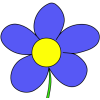
\includegraphics[width=0.3\textwidth]{graphics/mygraphic2.png}
%   \else
%     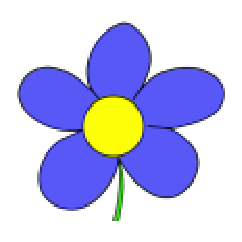
\includegraphics[width=0.3\textwidth]{graphics/mygraphic2-for-ps.eps}
%   \fi
%   \caption{A Flower.}
% \end{figure}


% Back Matter
% ------------

% The following command will typeset the bibliography,
% then typeset the Hebrew part of the thesis:
% - Cover page
% - Title page
% - Acknowledgements page
%  (NO table of contents or list of figures in Hebrew)
% - (Extended) abstract (1000-2000 words)
%
% based on information you've provided in the thesis-fields file
% (including the relative paths to your bib files). The Hebrew
% content will be typeset in _reverse_page_order_, i.e. first
% in the file will be the last page of the abstract, and the
% Hebrew cover page will be the last page of the file.
%
\makebackmatter

% The resulting PDF can be printed and taken straight to binding,
% i.e. you do not need to flip any pages anywhere. Of course,
% mind the LaTeX error and warning messages, overfull hboxes etc.

\end{document}

